\documentclass{article}
\usepackage{graphicx}
\usepackage[margin=1in]{geometry}
\usepackage{hyperref}
\usepackage{placeins}

\newcommand{\Csharp}{%
  {\settoheight{\dimen0}{C}C\kern-.05em \resizebox{!}{\dimen0}{\raisebox{\depth}{\#}}}}

\begin{document}
\title{COMP6205 Web Development\\}
\author{Group 8\\Shantnu Singh - ss18g15\\Doug Morgan - dm3g14}
\date{\today}
\maketitle

\section{Overview}
    \paragraph{}
        The assignment involved creating a prototype for a real-estate website aimed at university students.
        The website needs to allow: landlords to list properties, administrators to approve properties, landlords to be able to track the status of their property, and students to view approved properties.
        We have achieved all of these requirements and have added a number of other useful features, including but not limited to landlords having the ability to edit any details of a property, requiring re-approval by the University officer.

    \paragraph{}
        We decided to call our website HelloHomes.

    \paragraph{}
        Since the project required efficient use of ASP.NET Razor pages, a technology neither of us had previously used, we decided to begin the project by pair programming, which allowed us to gain an understanding of how the logic of the application would work, and then develop individually later on, each of us working on a set of features.
        This meant that tasks could easily be split between us.

    \paragraph{}
        To make programming separately easier, we used Git for version control.
        Visual Studio 2017 was the ideal IDE as it had in-build Razor development support, such as; IntelliSense, for code completion; package management, through NuGet and deployment to Azure.
        An SQL Express database was used and initialised through migrations created using the IDE.

\FloatBarrier
\section{Design}
    \paragraph{}
        Before we could start programming, some thought had to be given to the design of the user interface and database.
        We did this on pen and paper and using tools such as LucidChart.
        The logo for the website was also created at this time and other images we used were sourced from the copyright-free section of Google Images.
        The initial design of the website and the final database design is shown in Figures \ref{fig:early_sketches} and \ref{fig:sql_tables}.

        \begin{figure}[ht]
            \centering
            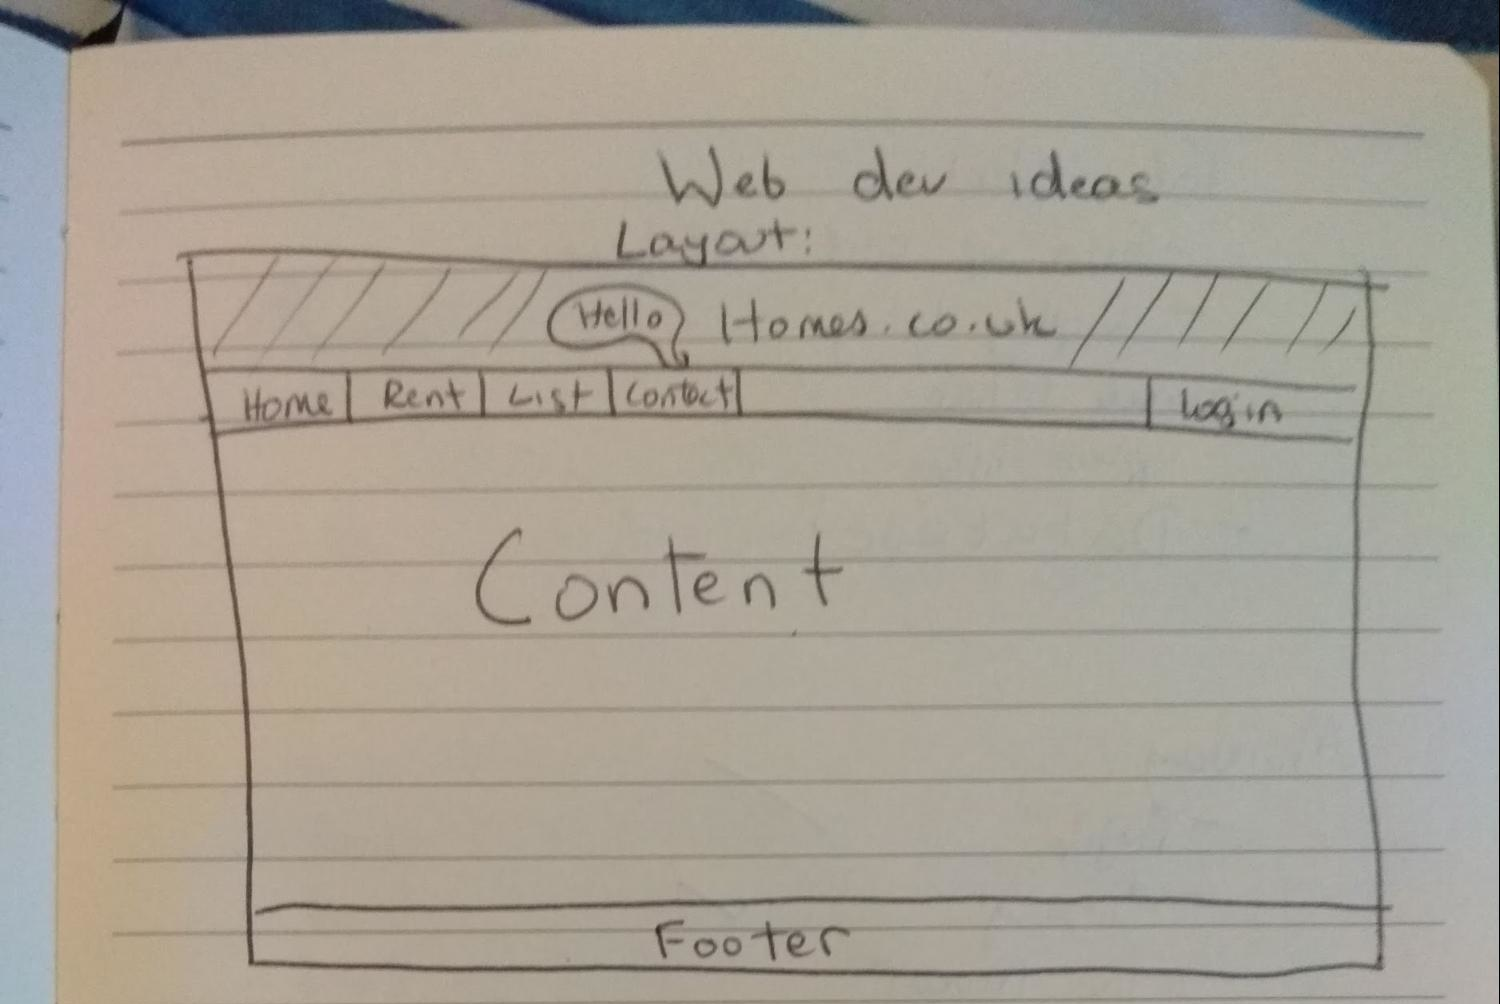
\includegraphics[width=0.48\textwidth]{figures/layout_sketch1.png}
            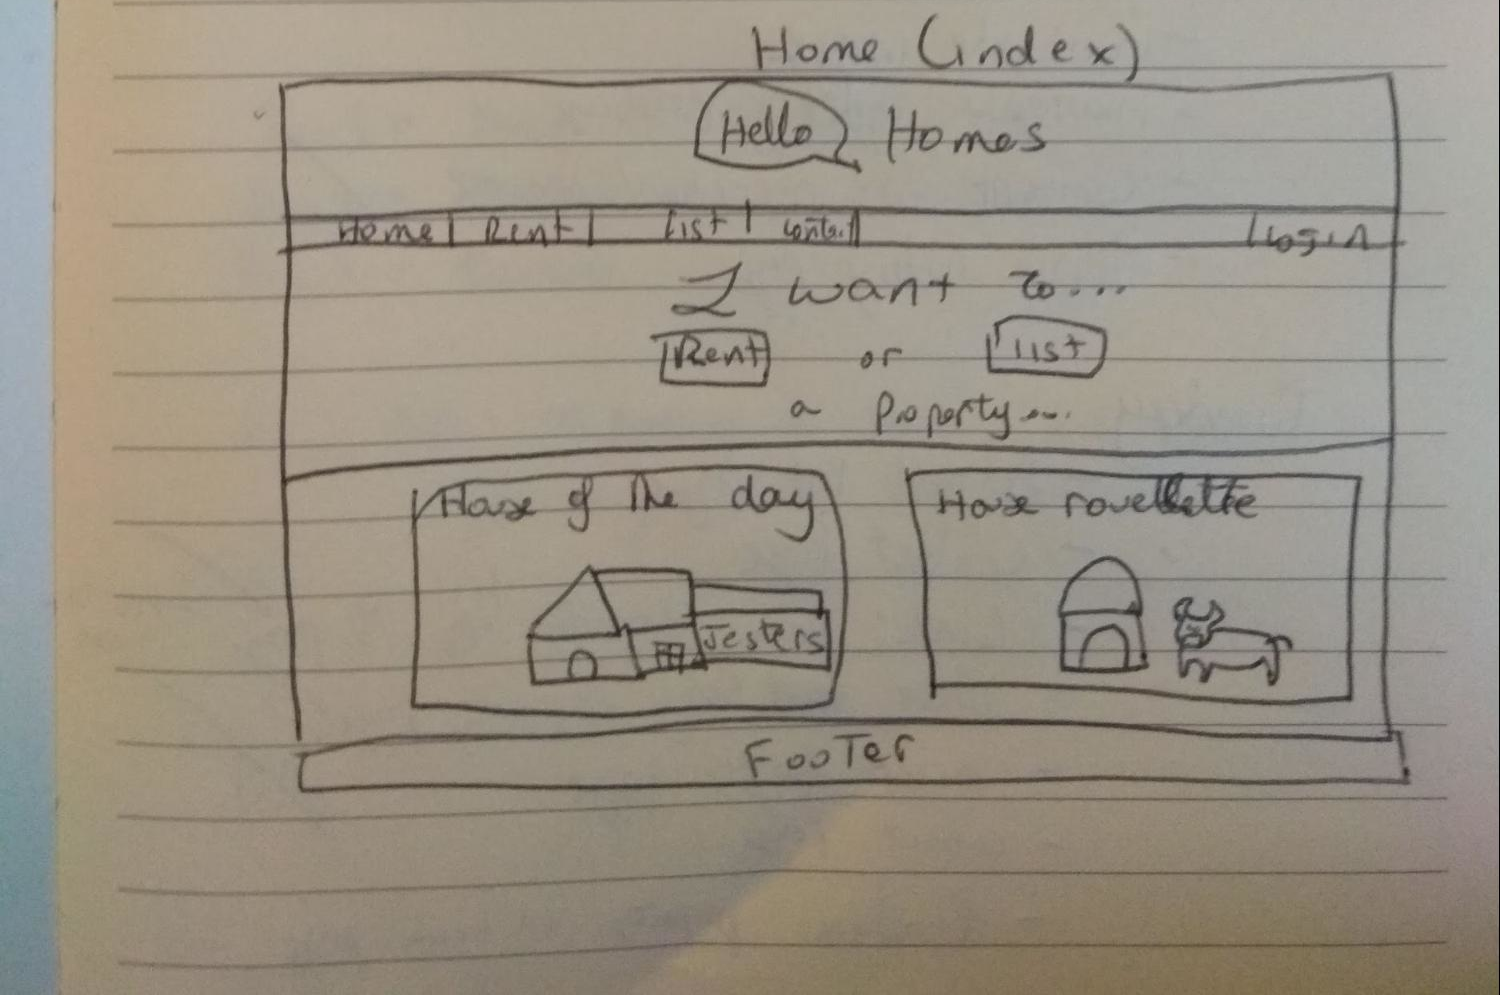
\includegraphics[width=0.48\textwidth]{figures/layout_sketch2.png}
            \caption[Early Sketches]{Early sketches of the web interface}
            \label{fig:early_sketches}
        \end{figure}

        \begin{figure}[ht]
            \centering
            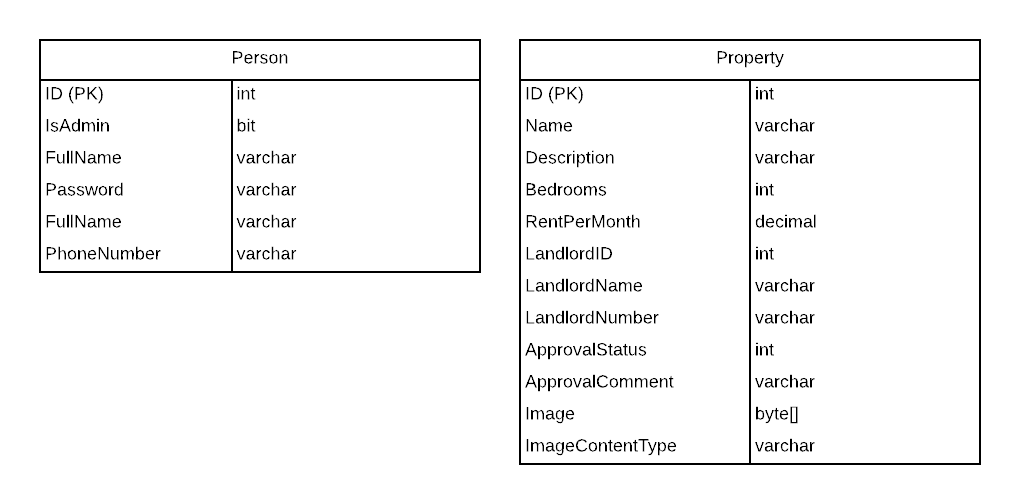
\includegraphics[width=0.8\textwidth]{figures/sql_tables.png}
            \caption[SQL Tables]{Tables used in the final SQL database}
            \label{fig:sql_tables}
        \end{figure}

    \paragraph{}
        When designing user accounts, consideration was given to all site users having an account, with different authorisation levels representing student, landlord and administrator.
        However, the student never needs to interact with the site in a way that would benefit from being logged into it, so it seemed more sensible to limit to only two kinds of user account: user and admin.
        A signed in user is able to post and edit property listings, and to see the approval status of their listings.
        An admin is able to approve or reject listings, and are required to give a brief comment in either case.
        Users who are not signed in have no capability to list properties or to view properties that have not been approved.

    \paragraph{}
        The visual design has been achieved using Bootstrap, an HTML and CSS library which provides dynamically resizable elements.
        We chose this tool for greater visual consistency over manually defined parameters, as it allows portable layouts to be defined easily, so that the site can be effectively viewed on all devices.

        \begin{figure}[!htb]
            \centering
            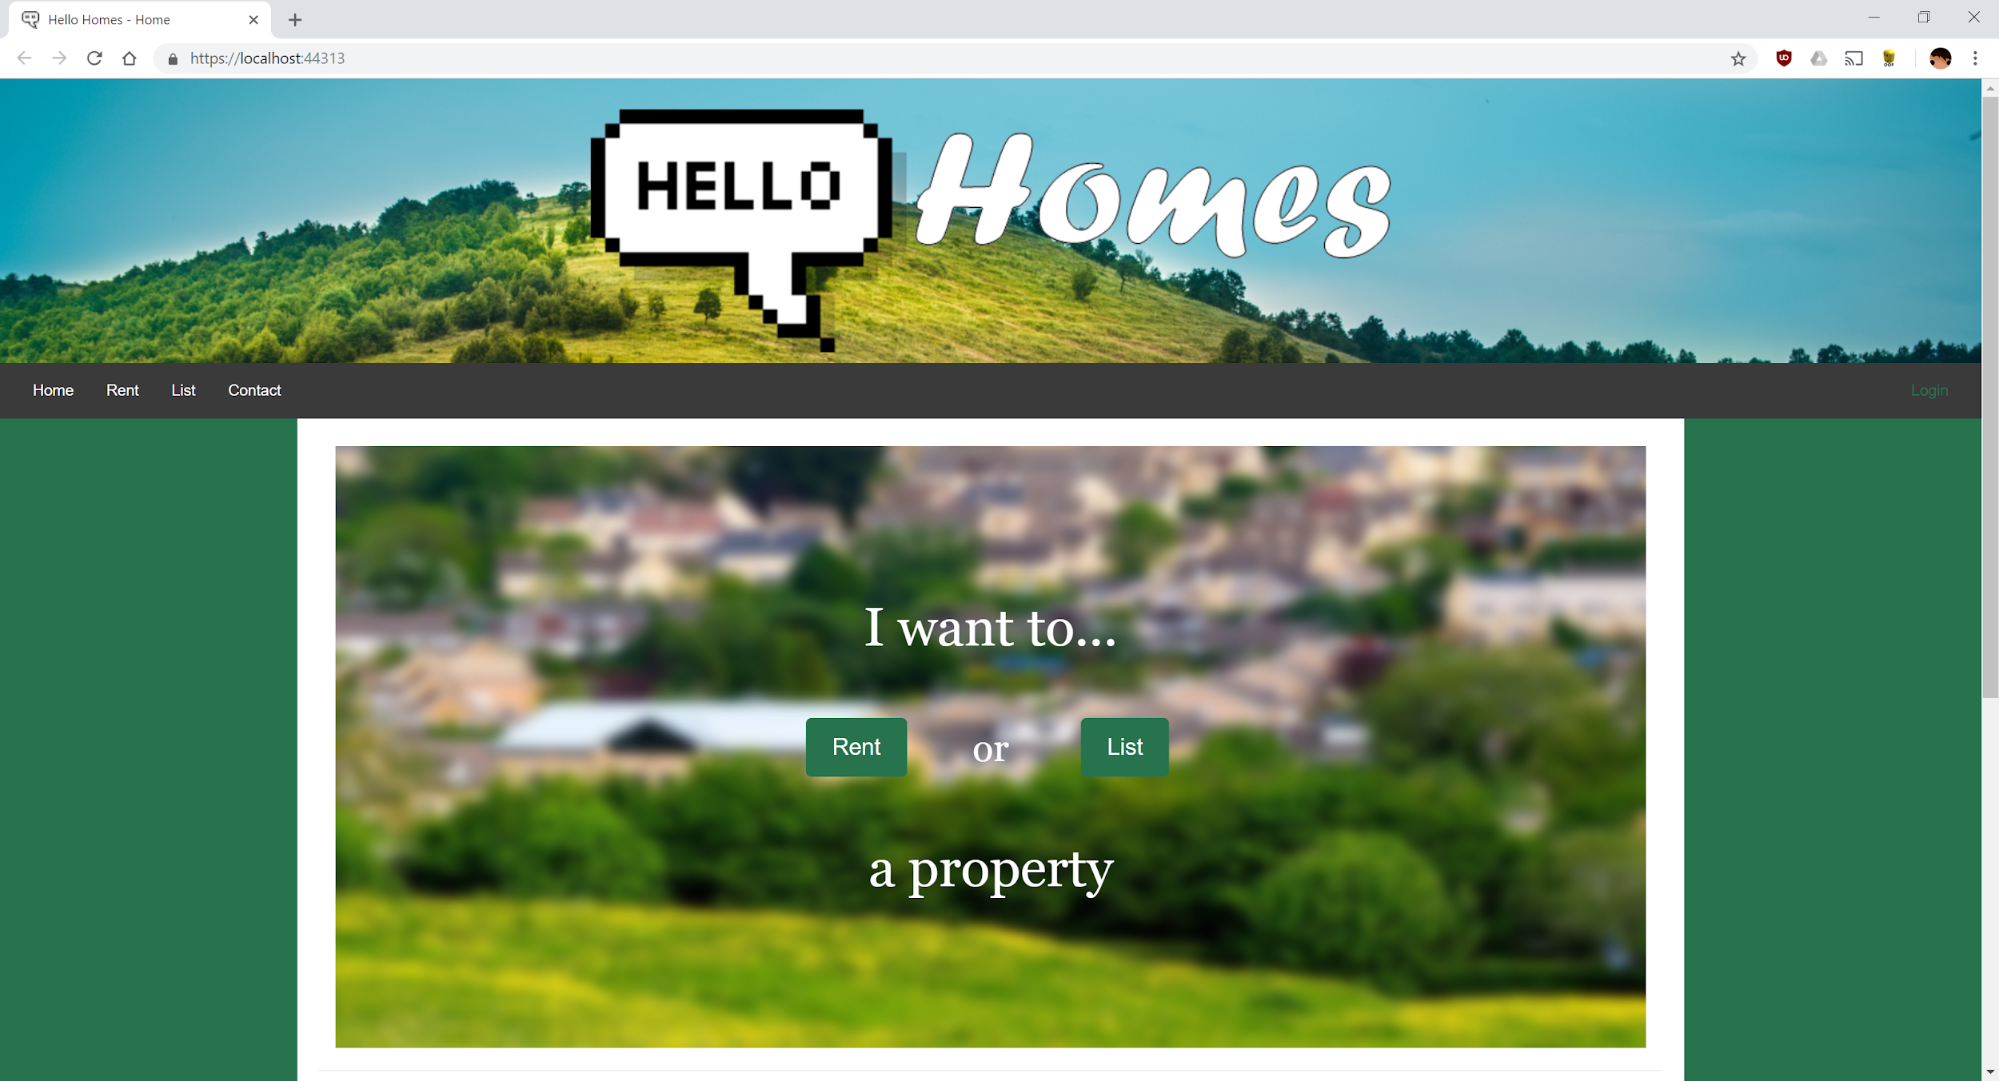
\includegraphics[width=0.8\textwidth]{figures/index_page.png}
            \caption[Home page layout]{Layout of the home page, designed using Bootstrap}
            \label{fig:index_page}
        \end{figure}

    \paragraph{}
        Throughout the project we used a highly graphical approach to the design. This was done to enhance visual feedback to the user by limiting the amount of reading that needs to be done. An example of this is the property listing page where the approval status of the property is displayed using “emojis” instead of text. This is evidenced below (Figure \ref{fig:emoji_status}).

        \begin{figure}[!htb]
            \centering
            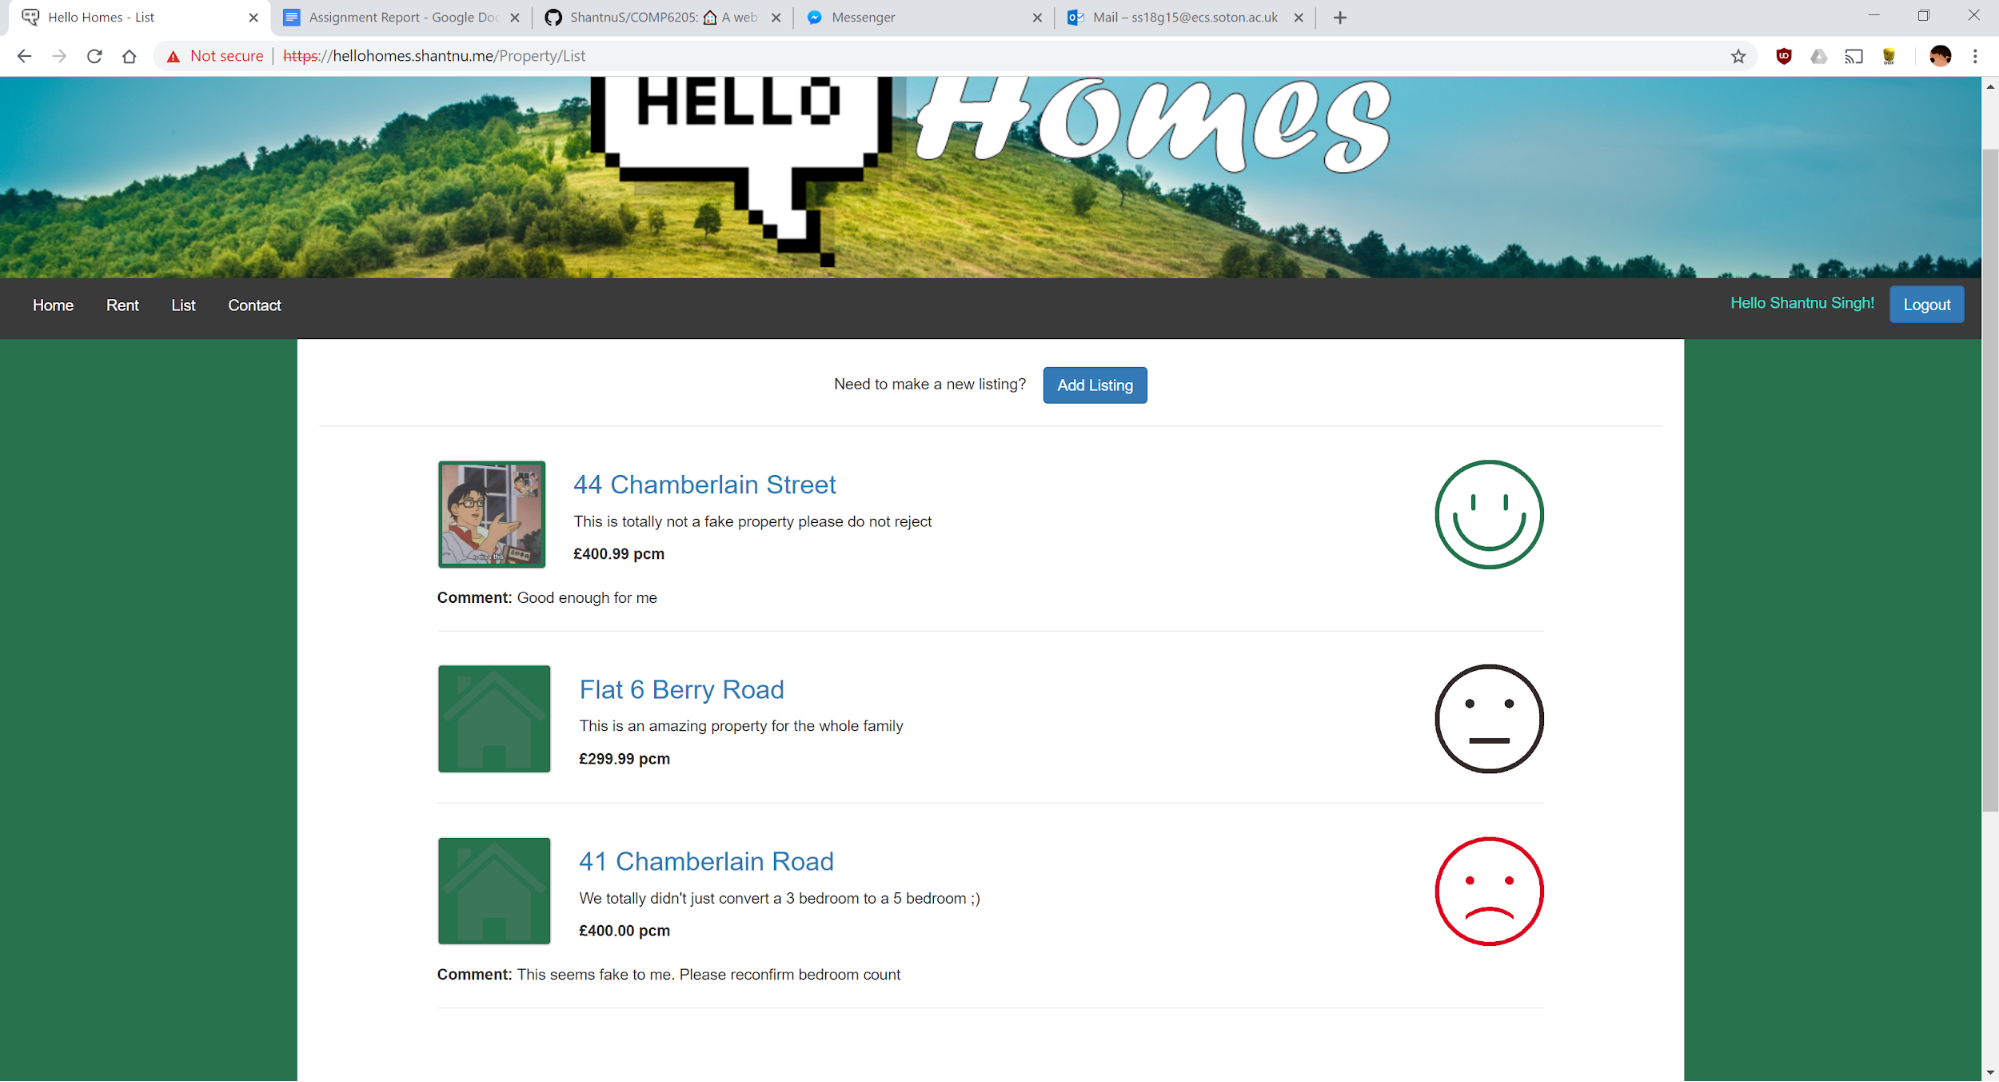
\includegraphics[width=0.8\textwidth]{figures/emoji_status.png}
            \caption[Emoji Status]{Using different emojis to represent approval status}
            \label{fig:emoji_status}
        \end{figure}

\FloatBarrier
\section{Features}
    \subsection{Main Features}
        \paragraph{}
            The main features of the website consisted of:
            \begin{itemize}\itemsep 0pt
                \item Ability for all users to view approved properties
                \item Ability for landlords to add new properties
                \item Ability for admins to approve and reject properties
            \end{itemize}

        \paragraph{}
            In addition to this, there had to be some form of authentication and a separate section for the admin user.

        \paragraph{}
            Figure \ref{fig:rent_page} shows the page where approved properties are listed.
            Here only the title, image, description and cost of the property is shown, but upon clicking the title of the property, the user is taken to a page where full details, including contact details are shown.

            \begin{figure}[!htb]
                \centering
                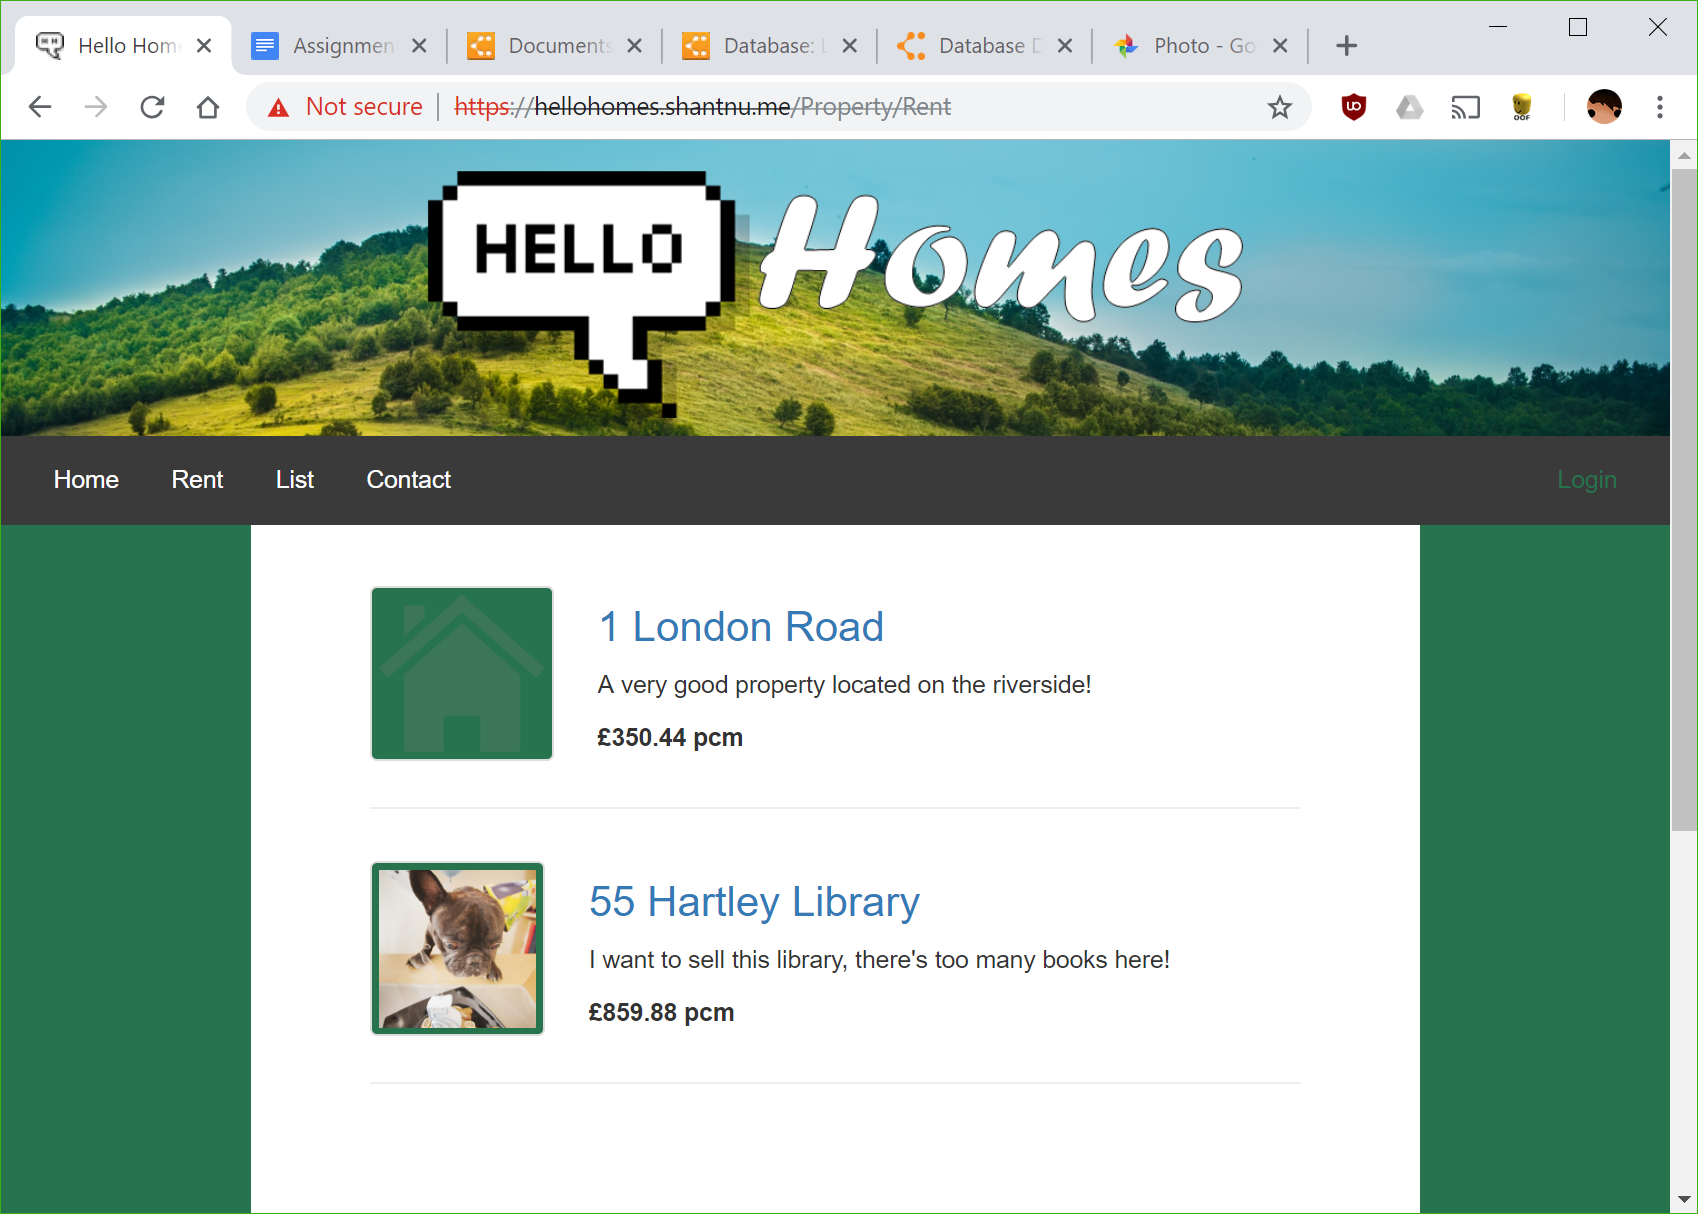
\includegraphics[width=0.7\textwidth]{figures/rent.png}
                \caption[Rent Page]{The rent page, where approved properties appear}
                \label{fig:rent_page}
            \end{figure}

        \paragraph{}
            The user, after authenticating, can access a page where they can see the properties they have listed and their current approval status.
            They are also shown a comment if the property was approved or rejected.
            On top of this page, there is a button to add a new property.
            Figure \ref{fig:add_property} shows the add property page.

            \begin{figure}[!htb]
                \centering
                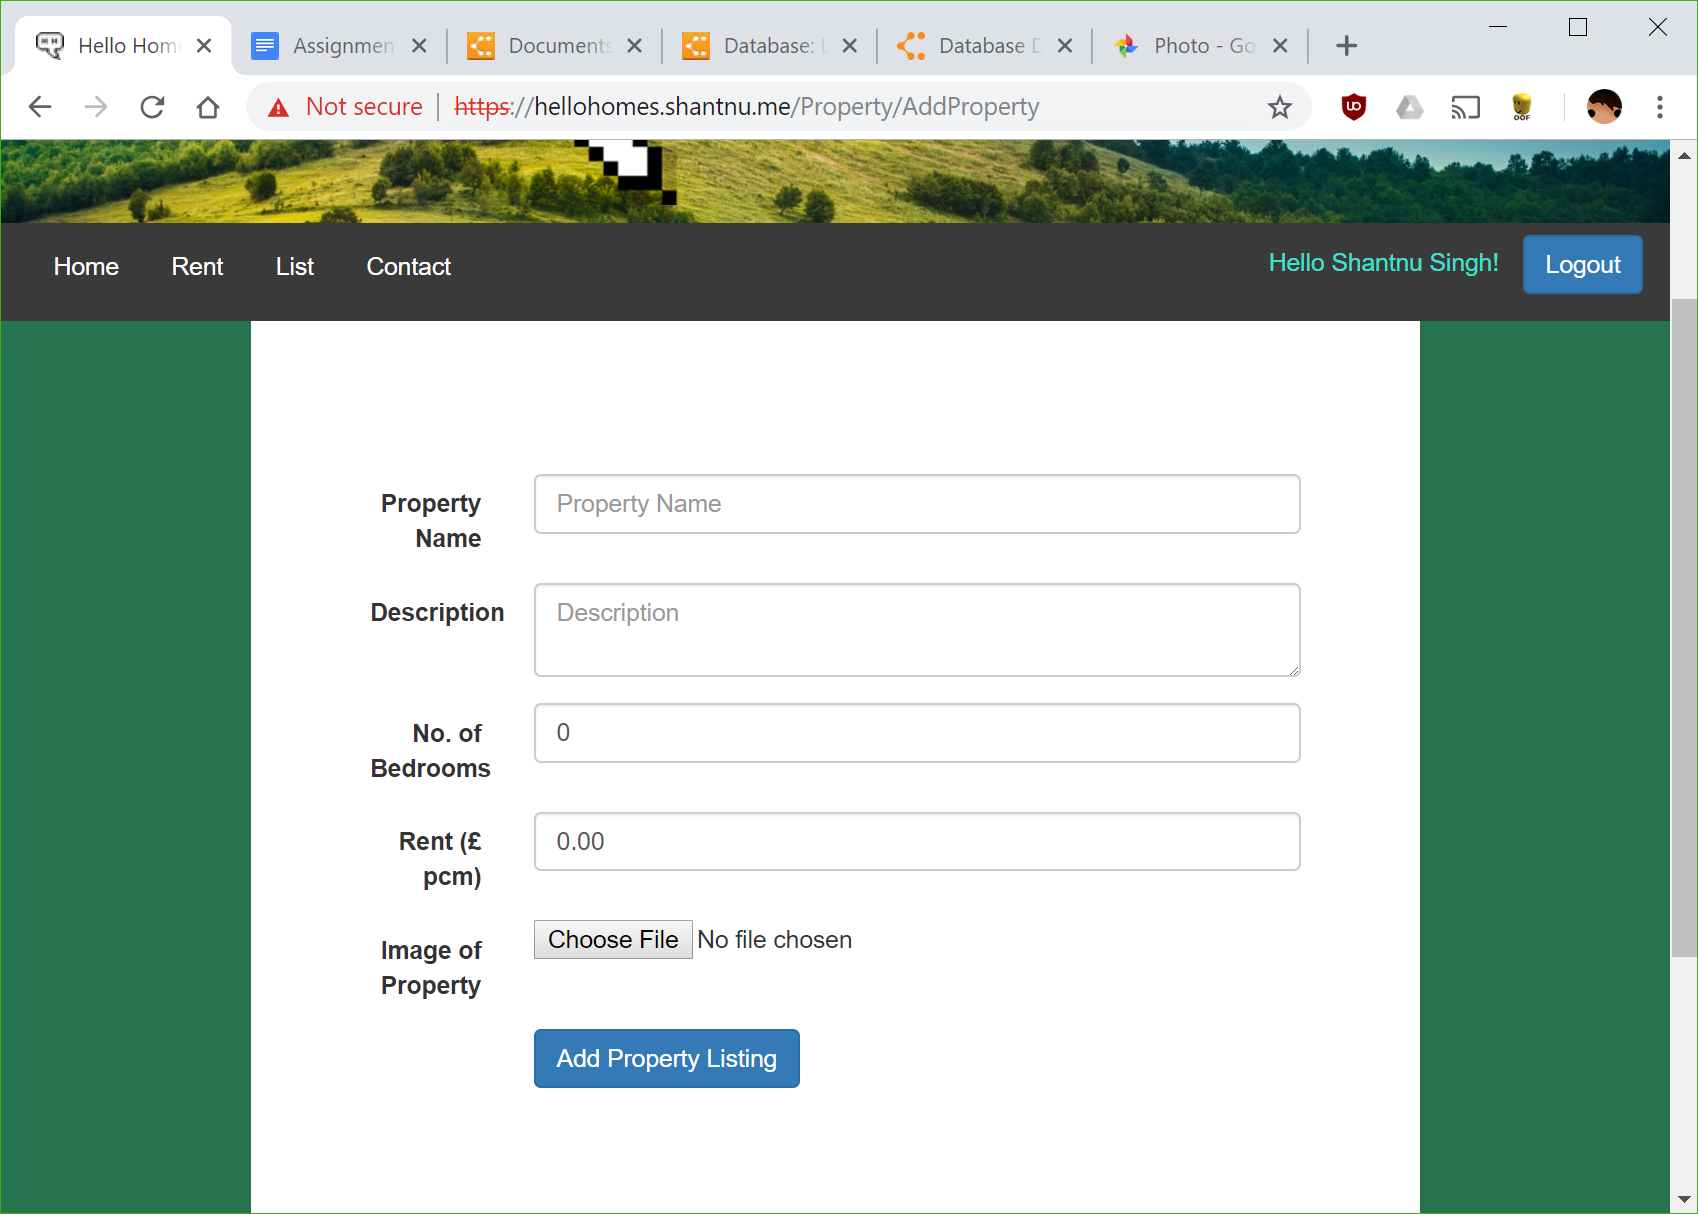
\includegraphics[width=0.7\textwidth]{figures/add_property.png}
                \caption[Add Property]{Adding a property to the listings}
                \label{fig:add_property}
            \end{figure}

        \paragraph{}
            When a new property is listed (or a current property edited), it must be approved before it is displayed; this can be done in the admin section of the site.
            Each pending property is listed here, along with a button to approve or reject them, as shown in Figure \ref{fig:admin_page}.
            Clicking on either of these options shows the admin details about the property, along with a text box to leave a comment regarding their decision, demonstrated in Figure \ref{fig:admin_approval}.

            \begin{figure}[!htb]
                \centering
                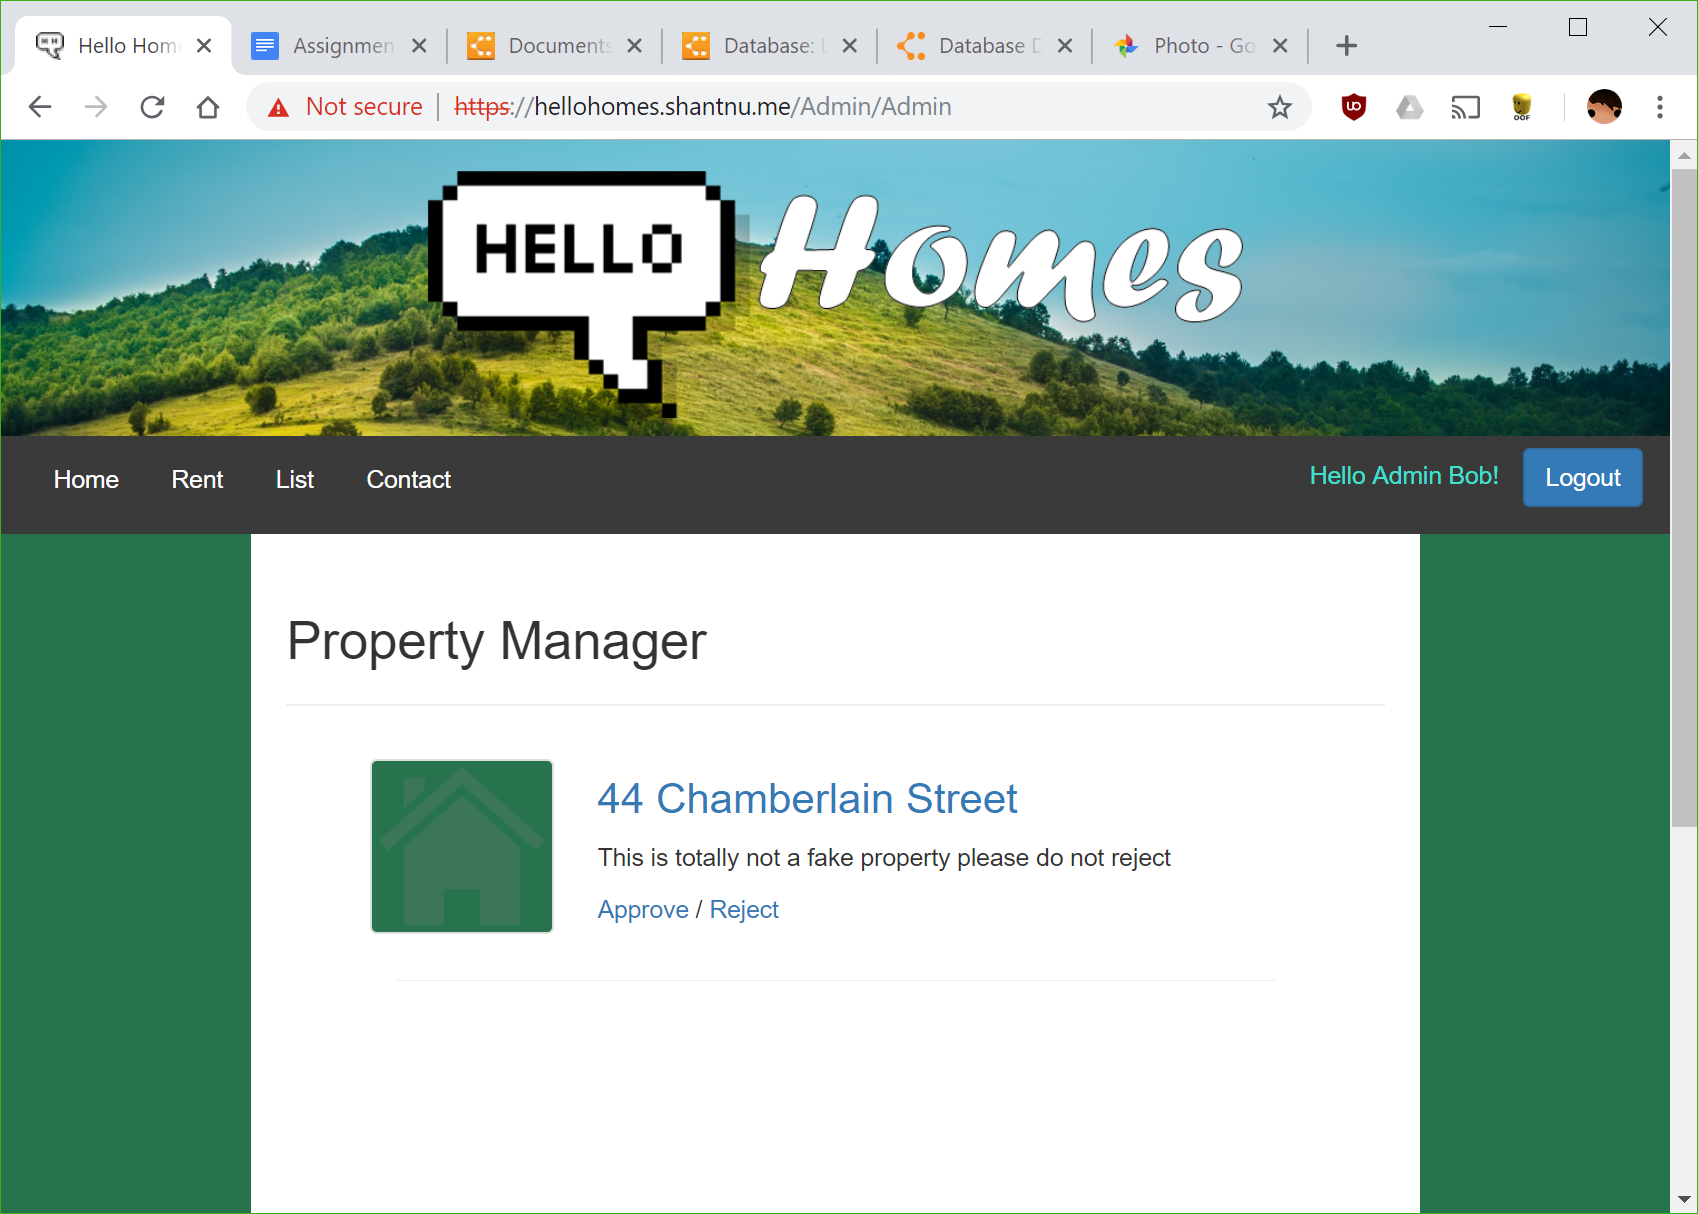
\includegraphics[width=0.7\textwidth]{figures/admin_page.png}
                \caption[Approve Property]{Admin viewing property listing for approval}
                \label{fig:admin_page}
            \end{figure}

            \begin{figure}[!htb]
                \centering
                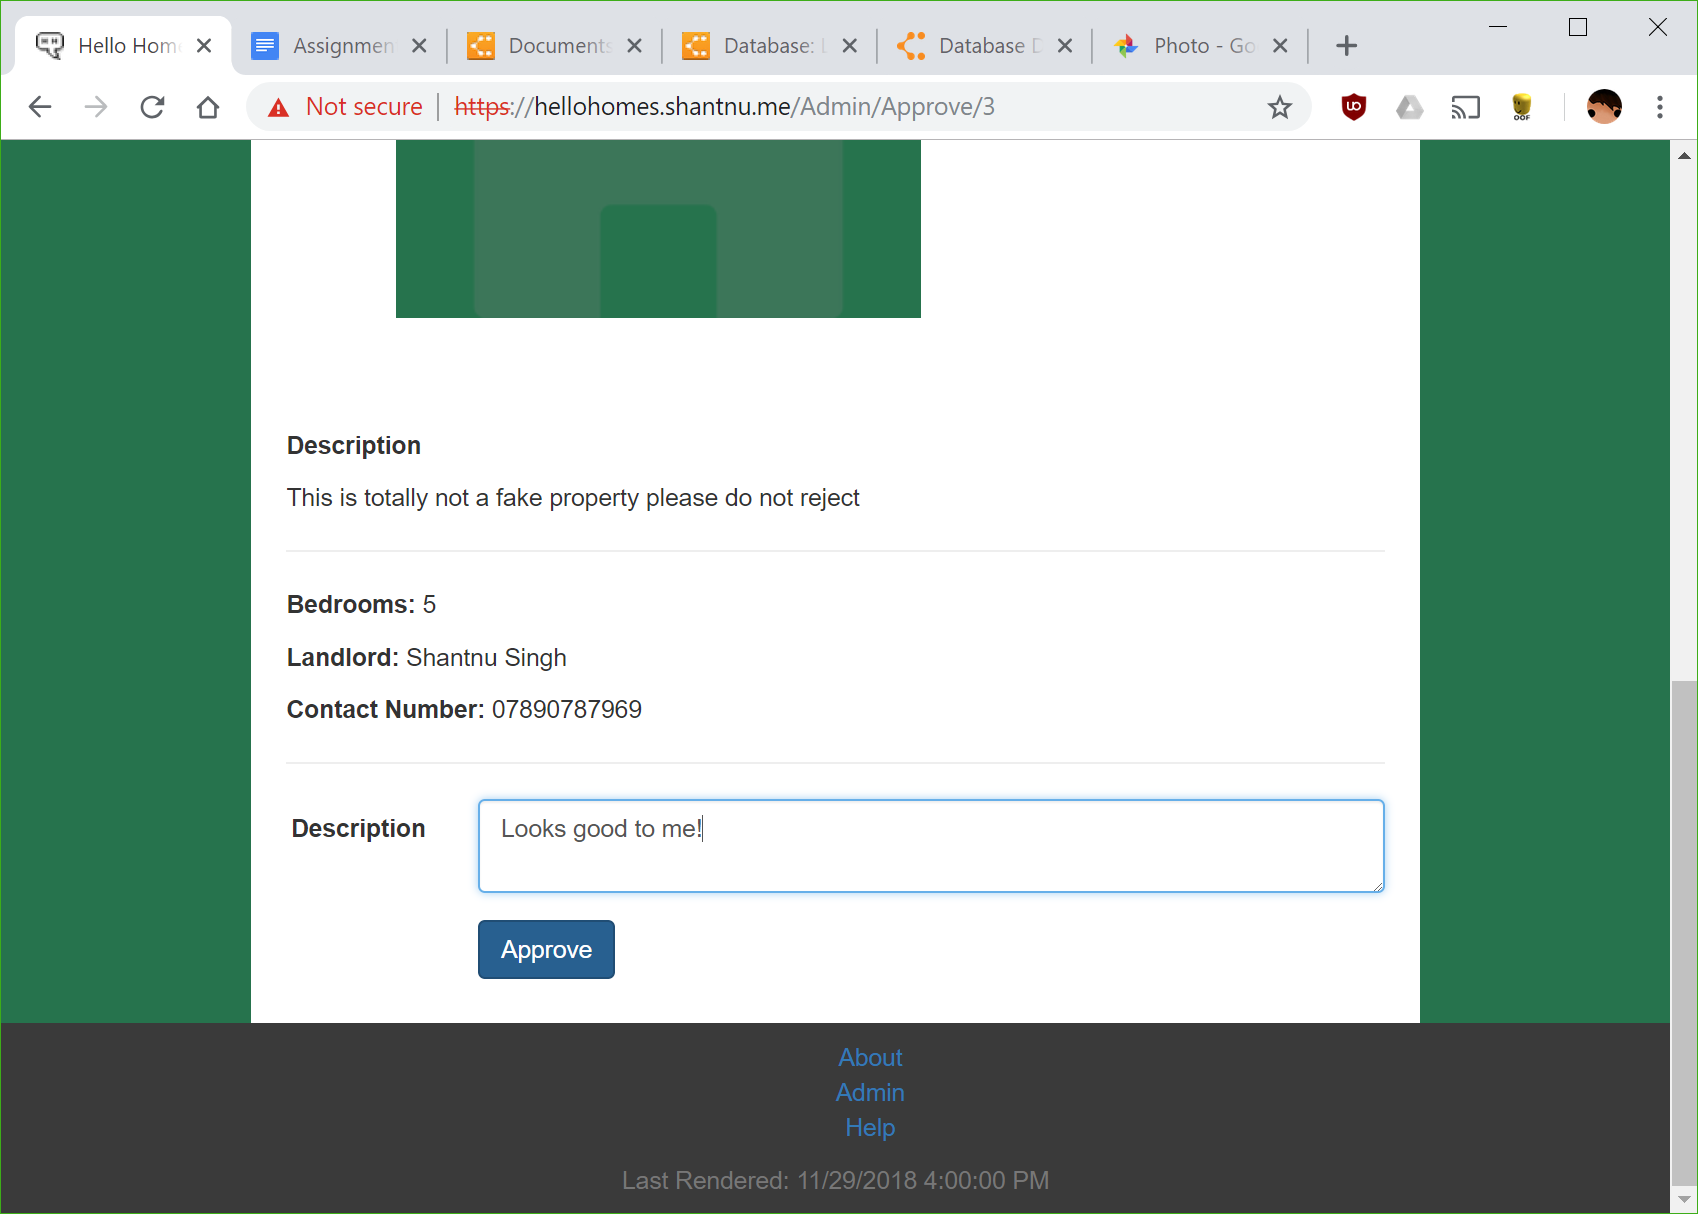
\includegraphics[width=0.7\textwidth]{figures/admin_approval.png}
                \caption[Comment on Property]{Admin approval or rejection comment}
                \label{fig:admin_approval}
            \end{figure}

        \paragraph{}
            Only the landlord and admin have to be authenticated.
            This is done by adding authorisation to certain pages of the site, so that the user has to login before accessing them.
            There is provisioning for this in ASP.NET.
            When the user logs in, they are authenticated via details stored in the database and a cookie session is created.
            This cookie can be used to see which user is logged in throughout the session and to determine if they are allowed to view certain pages.

    \subsection{Additional Features}
        \paragraph{}
            On top of the core functionality, we implemented some additional features to the site.
            These were done to demonstrate our understanding of Razor web development and to test its limitations.

        \paragraph{}
            Firstly, we added the option to edit properties.
            If the user views a property they themselves listed, the are shown a button on top of the page which allows them to edit the property.
            Doing this takes them to a page similar to the new property page, except the previous details are filled in.
            They can simply change any information and re-list the site.
            However, doing this means the approval status is reset.
            This was done to prevent a malicious landlord changing details after being approved, but to also allow them to act on the comments left by the admin.

            \begin{figure}[!htb]
                \centering
                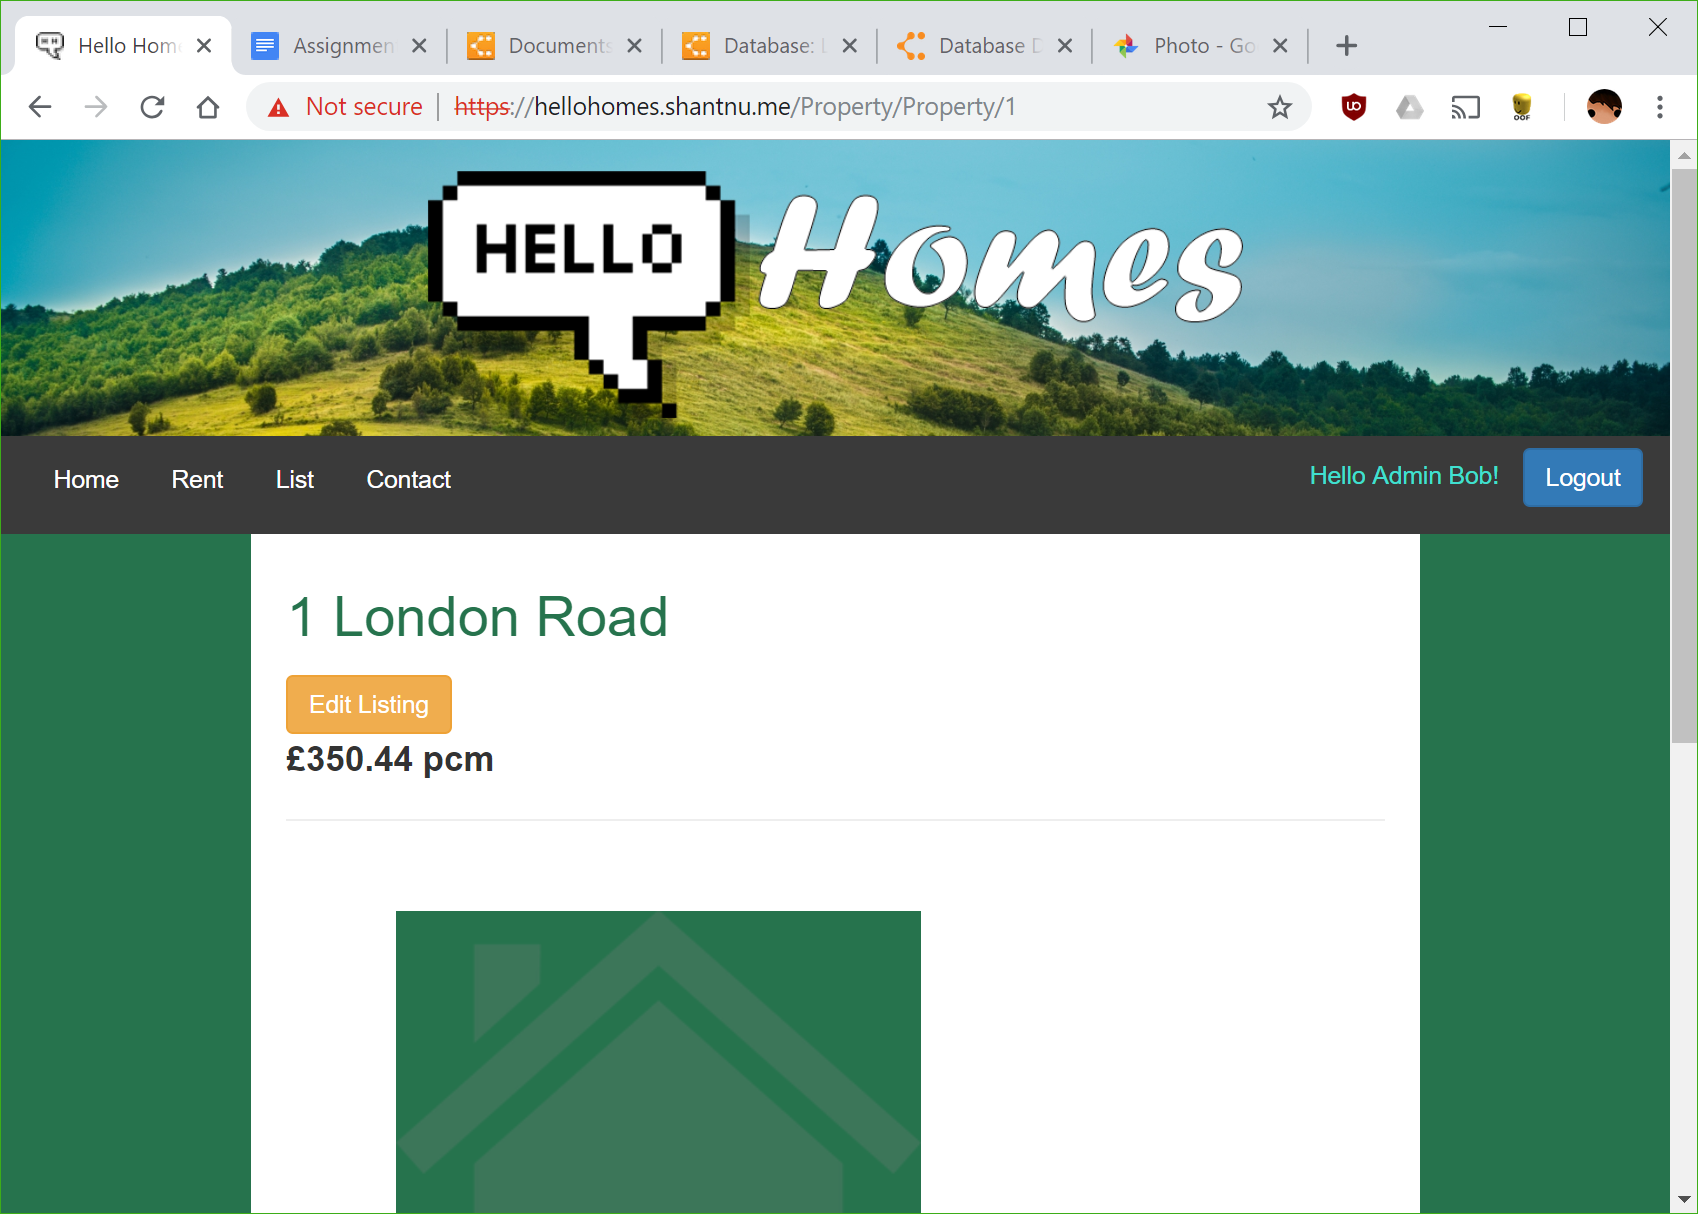
\includegraphics[width=0.7\textwidth]{figures/edit_properties.png}
                \caption[Edit Properties]{The user is able to edit a property they own}
            \end{figure}

        \paragraph{}
            Since Razor pages allows \Csharp\space code to be run to pre-process a HTML page, we could use this to test some interesting features.
            On the homepage of the site, we display the “property of the day” and a “random property”.
            This is done by creating an array of all approved properties and choosing relevant ones for each section.
            For the property of the day, the result is based on the current day of the week and the number of approved properties, whereas the random property can be any approved property and changes upon refresh!

            \begin{figure}[!htb]
                \centering
                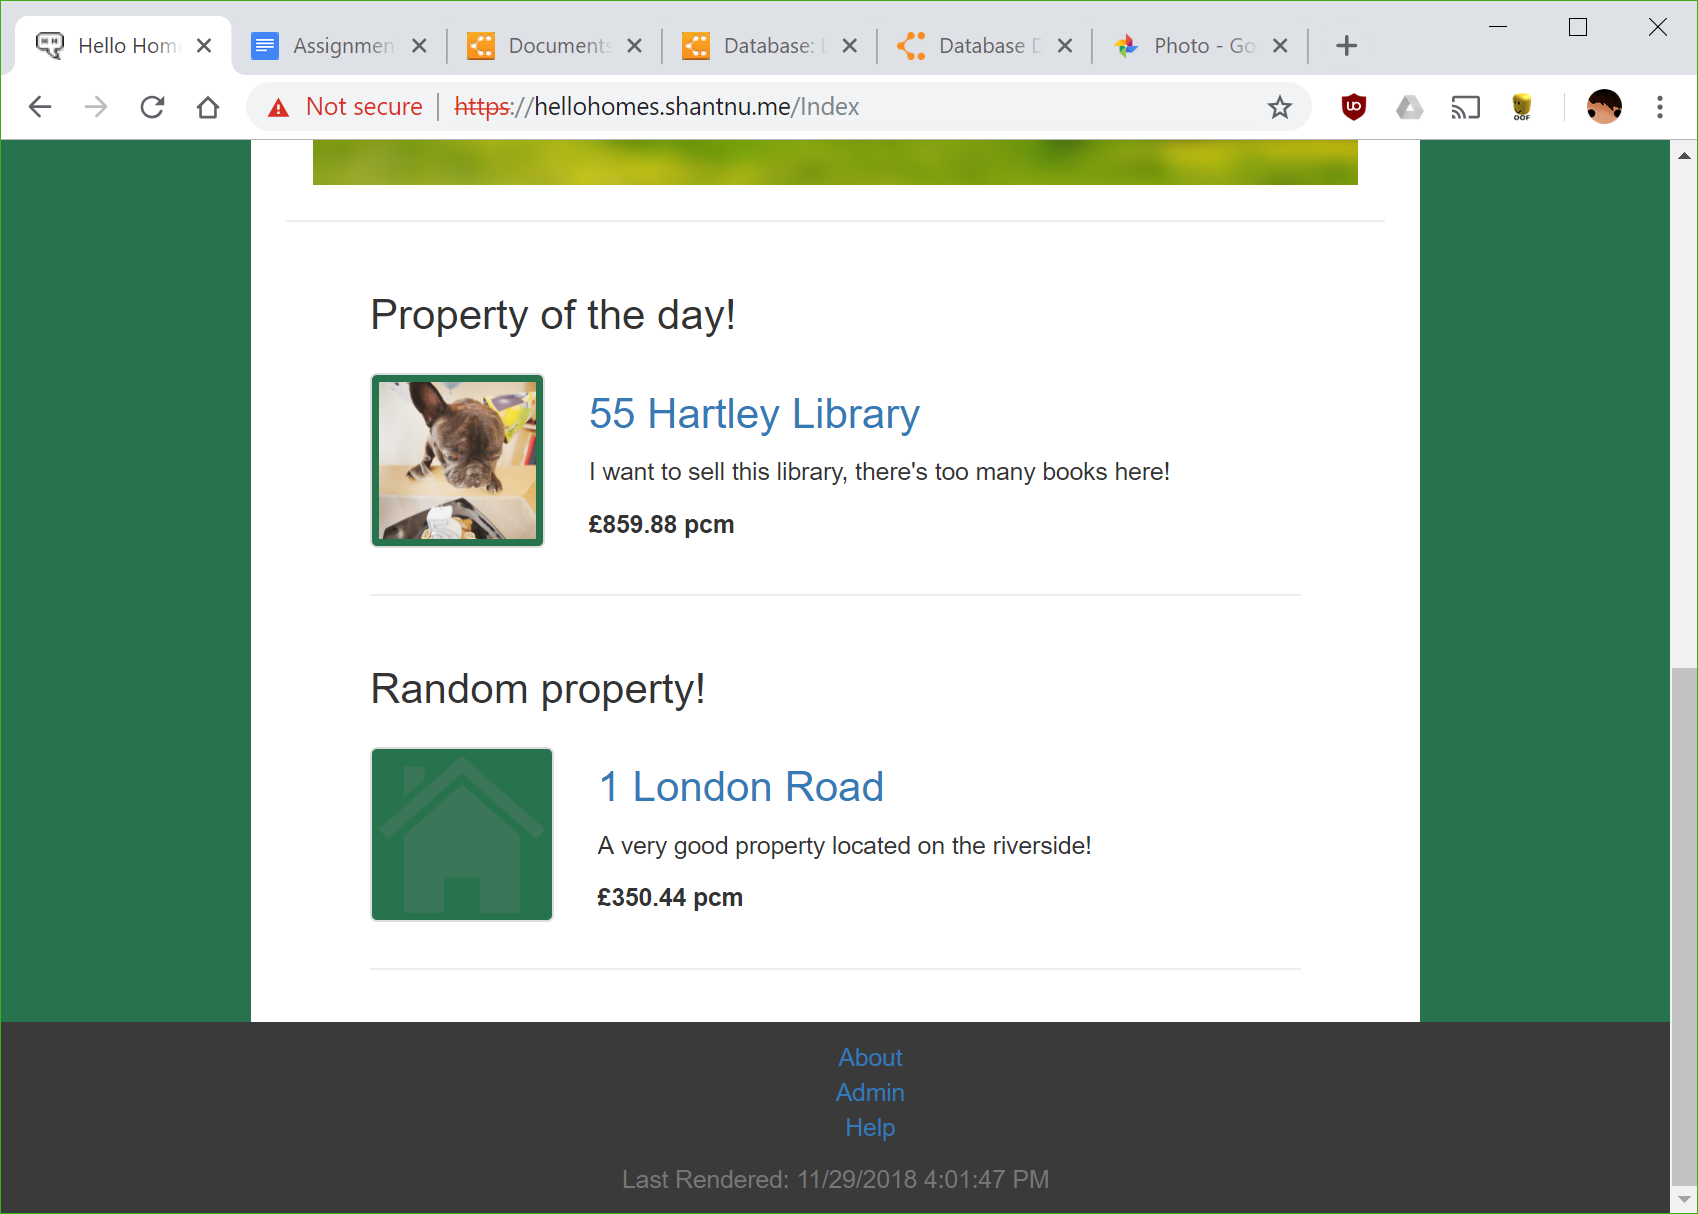
\includegraphics[width=0.7\textwidth]{figures/property_of_the_day.png}
                \caption[Property Of The Day]{The homepage displays the property of the day and a random property}
            \end{figure}

        \paragraph{}
            We also experimented with routing and displaying data relevant to the user in the site.
            For example, clicking the user’s name on the navigation bar, next to the logout button, takes the user to their profile page where their details are visible.
            In the future, we could add the ability to edit profiles and maybe add a profile picture.

        \paragraph{}
            A final example of additional features is embedding other services onto the website.
            On the contact page, we embedded a Google Maps applet which displays the location of the HelloHomes headquarters.
            Since HelloHomes is a fictional entity, we used the University's address.

            \begin{figure}[!htb]
                \centering
                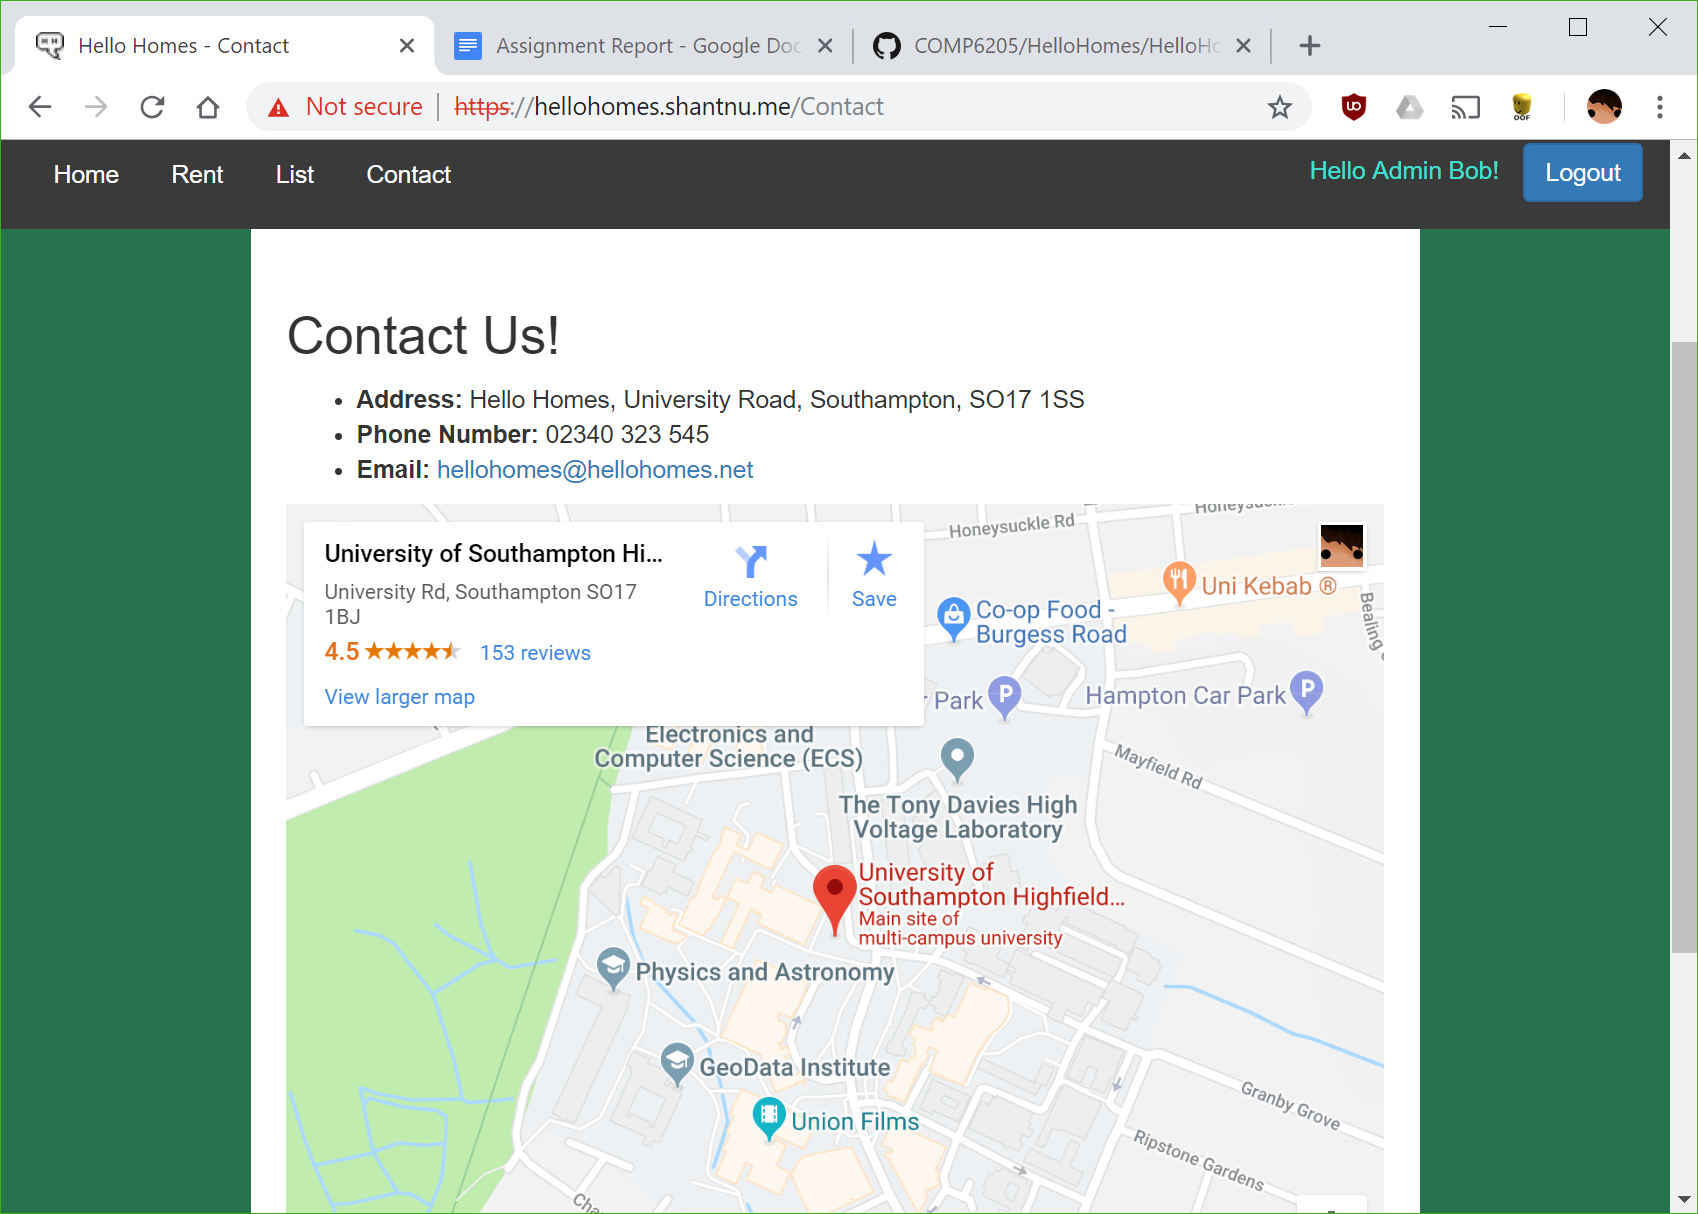
\includegraphics[width=0.7\textwidth]{figures/google_maps.png}
                \caption[Google Maps]{A Google Maps applet was embedded onto the contacts page}
            \end{figure}

    \subsection{Security}
        \paragraph{}
            Since we had done a number of cyber-security modules at the university, we thought it was important to consider the security aspects of the site.
            This also gave us the opportunity to evaluate the features provided by ASP.NET and Razor.

        \subsubsection{Password Hashing}
            \paragraph{}
                Since the password had to be stored in an SQL database, we thought it was unwise to store them in plain text.
                This is especially important as, for example, Visual Studio has an option to view data stored in the database.
                Therefore, we implemented password hashing to the website.
                This is done by creating a SHA-1 hash of the password before storing them to the database and then simply comparing the hash to a hashed version of the password entered by the user.
                The reason to use SHA-1 was due to its superiority to MD5 and simplicity to some other algorithms.
                However, in the future we would like to implement PBKDF2 or bscript as they are the systems recommended in the field.

        \subsubsection{Secure File Upload}
            \paragraph{}
                The only area of the site where the user could upload a file was when submitting an image along with the property.
                To combat this, we ensured the file input box only accepted image files with the MIME type for PNG or JPEG.
                This ensures that safe files are uploaded.
                To further improve this, the file size could be capped or the extension checked.

        \subsubsection{Built-in Security}
            \paragraph{}
                There were a number of security features that were built into the libraries we used from ASP.NET.
                Firstly, since the user was authenticated via cookies, it was important that a malicious individual could not alter the value of the cookie to gain access to another user’s account.
                Fortunately, cookies are automatically hashed by ASP.NET’s authentication library and thus such an attack cannot be carried out.

            \paragraph{}
                Secondly, Cross Site Request Forgery (CSRF) can be used to make malicious requests to the server from a user’s behalf.
                Razor pages come with built in verification to prevent this \cite{request_verification}.

            \paragraph{}
                Finally, when inputs are passed between the SQL database and the application, it is important to ensure they are sanitised to prevent SQL injection.
                Luckily, using the database context super-class when creating the database ensures this is done.
                This also protects the site against Cross-Site Scripting (XSS).

\FloatBarrier
\section{Testing}
    \subsection{Functionality Testing}
        \paragraph{}
            The databases were verified to be working as expected with the use of automatic seeding.
            Functions have been written in \texttt{SeedProperties.cs} and \texttt{SeedPeople.cs} to automatically add database entries on startup if there are none existing.
            This allowed us to test the functionality of most parts of the site before user login and property listing aspects were in place, which in turn allowed us to reduce the scope of our search for issues that arose while these elements were being programmed.

        \paragraph{}
            For other core functionalities, white-box testing was used extensively throughout development, both to ensure that each feature of the site had been robustly implemented and as part of our regression testing.
            This was extremely useful as it revealed several instances of changes made to files for a new feature affecting the performance of previously implemented elements.

        \paragraph{}

        \paragraph{}
            An example test case for editing listings is presented here:

            \begin{itemize}\itemsep 0pt
                \item Launch the site.
                \item Navigate to the listings page - this prompts logging in, which should be completed.
                \item Select a property listing.
                \item Select edit and upload a new image - save these changes.
                \item Ensure that the changes appear in the listings page and that no other changes have been made erroneously.
            \end{itemize}

    \subsection{Portability Testing}
        \paragraph{}
            Website portability is a big advantage of Razor pages. This along with bootstrap meant that the website should be compatible with different screen resolutions and sizes. Furthermore, the style-sheet for aspects of the front-end was written with relative values rather than absolute values to prevent issues with oversized objects.

        \paragraph{}
            Although during development we used Google Chrome to ensure the functionality of the website, below are screen-shots of the website in different screen sizes, browsers and devices, (figures \ref{fig:edge}, \ref{fig:firefox}, \ref{fig:android} and \ref{fig:small_display}). This could be done easily after deploying to Azure (this is detailed in extensions).

            \begin{figure}[!htb]
                \centering
                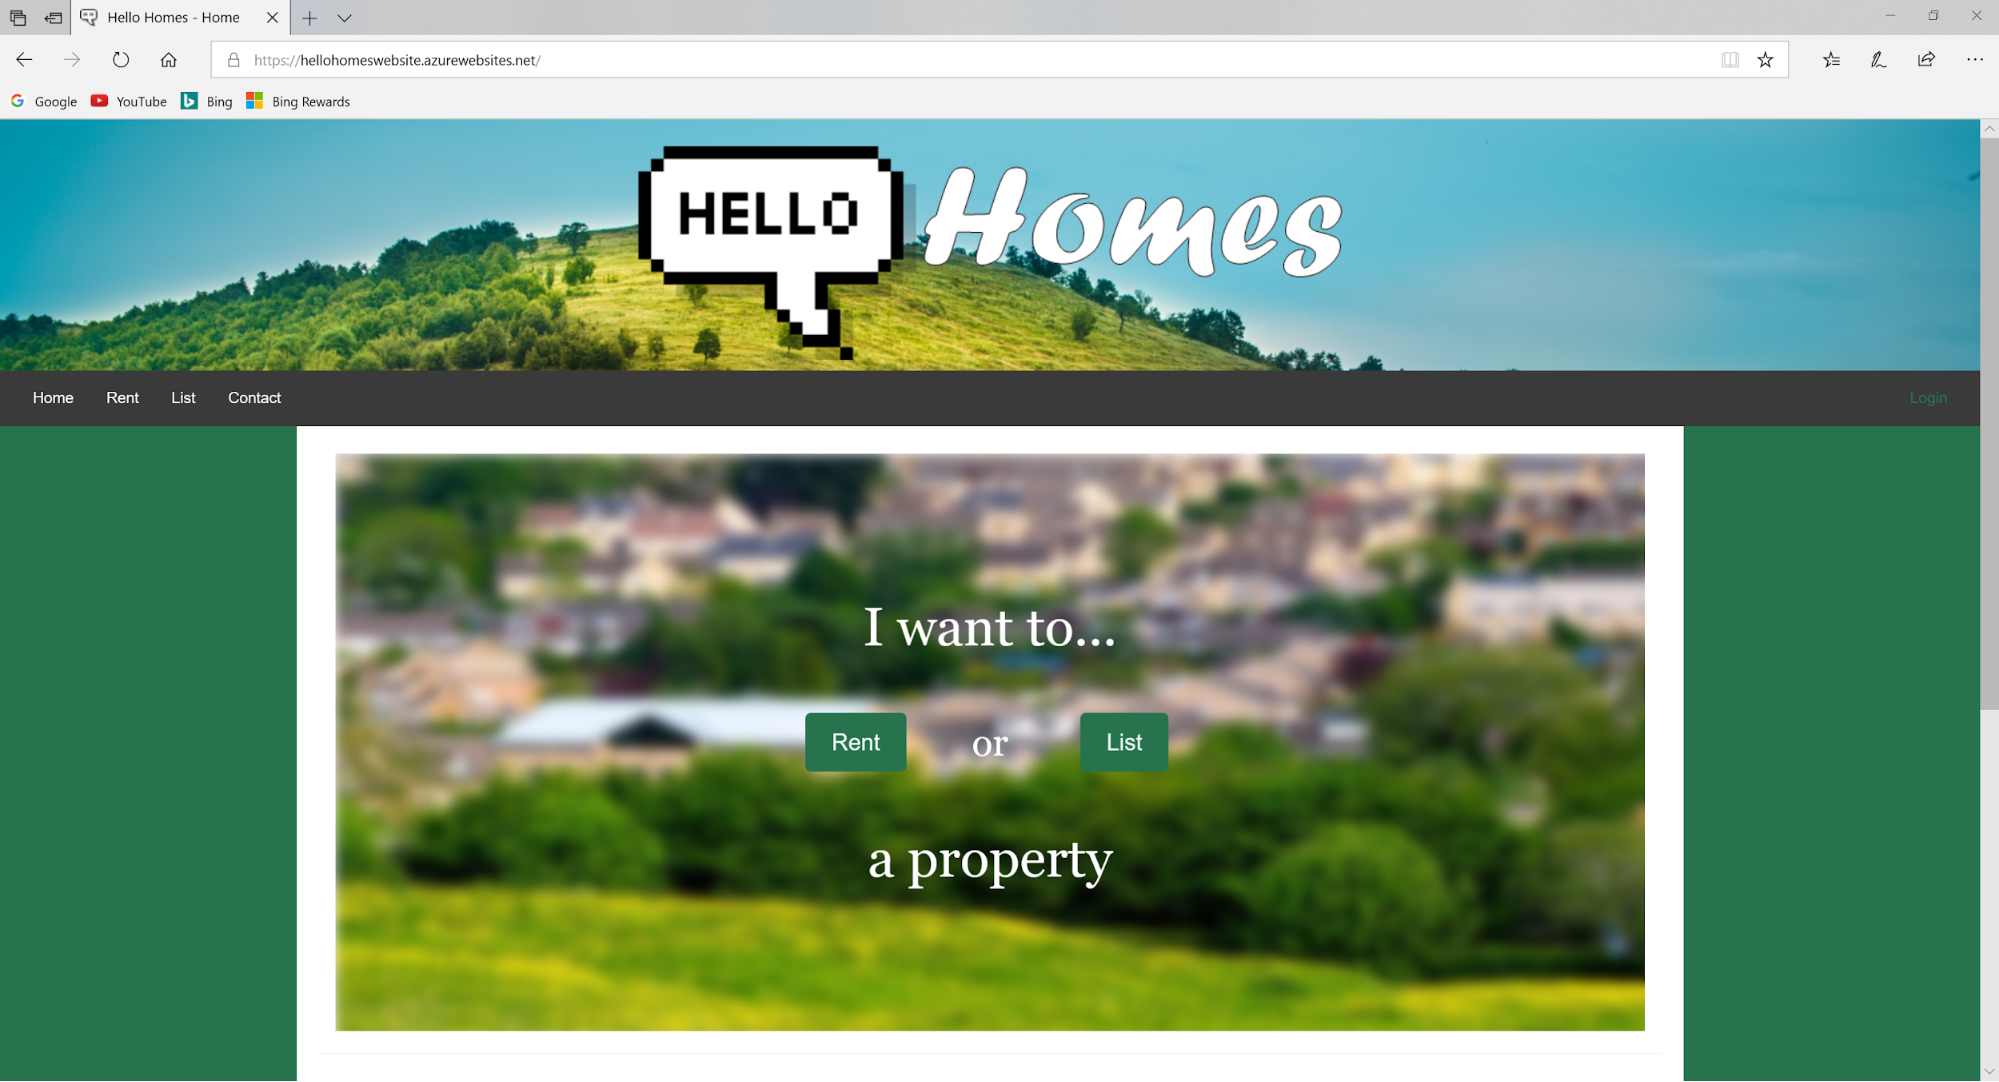
\includegraphics[width=0.8\textwidth]{figures/edge.png}
                \caption[Edge Scaling]{The performance was similar on Microsoft Edge}
                \label{fig:edge}
            \end{figure}

            \begin{figure}[!htb]
                \centering
                \frame{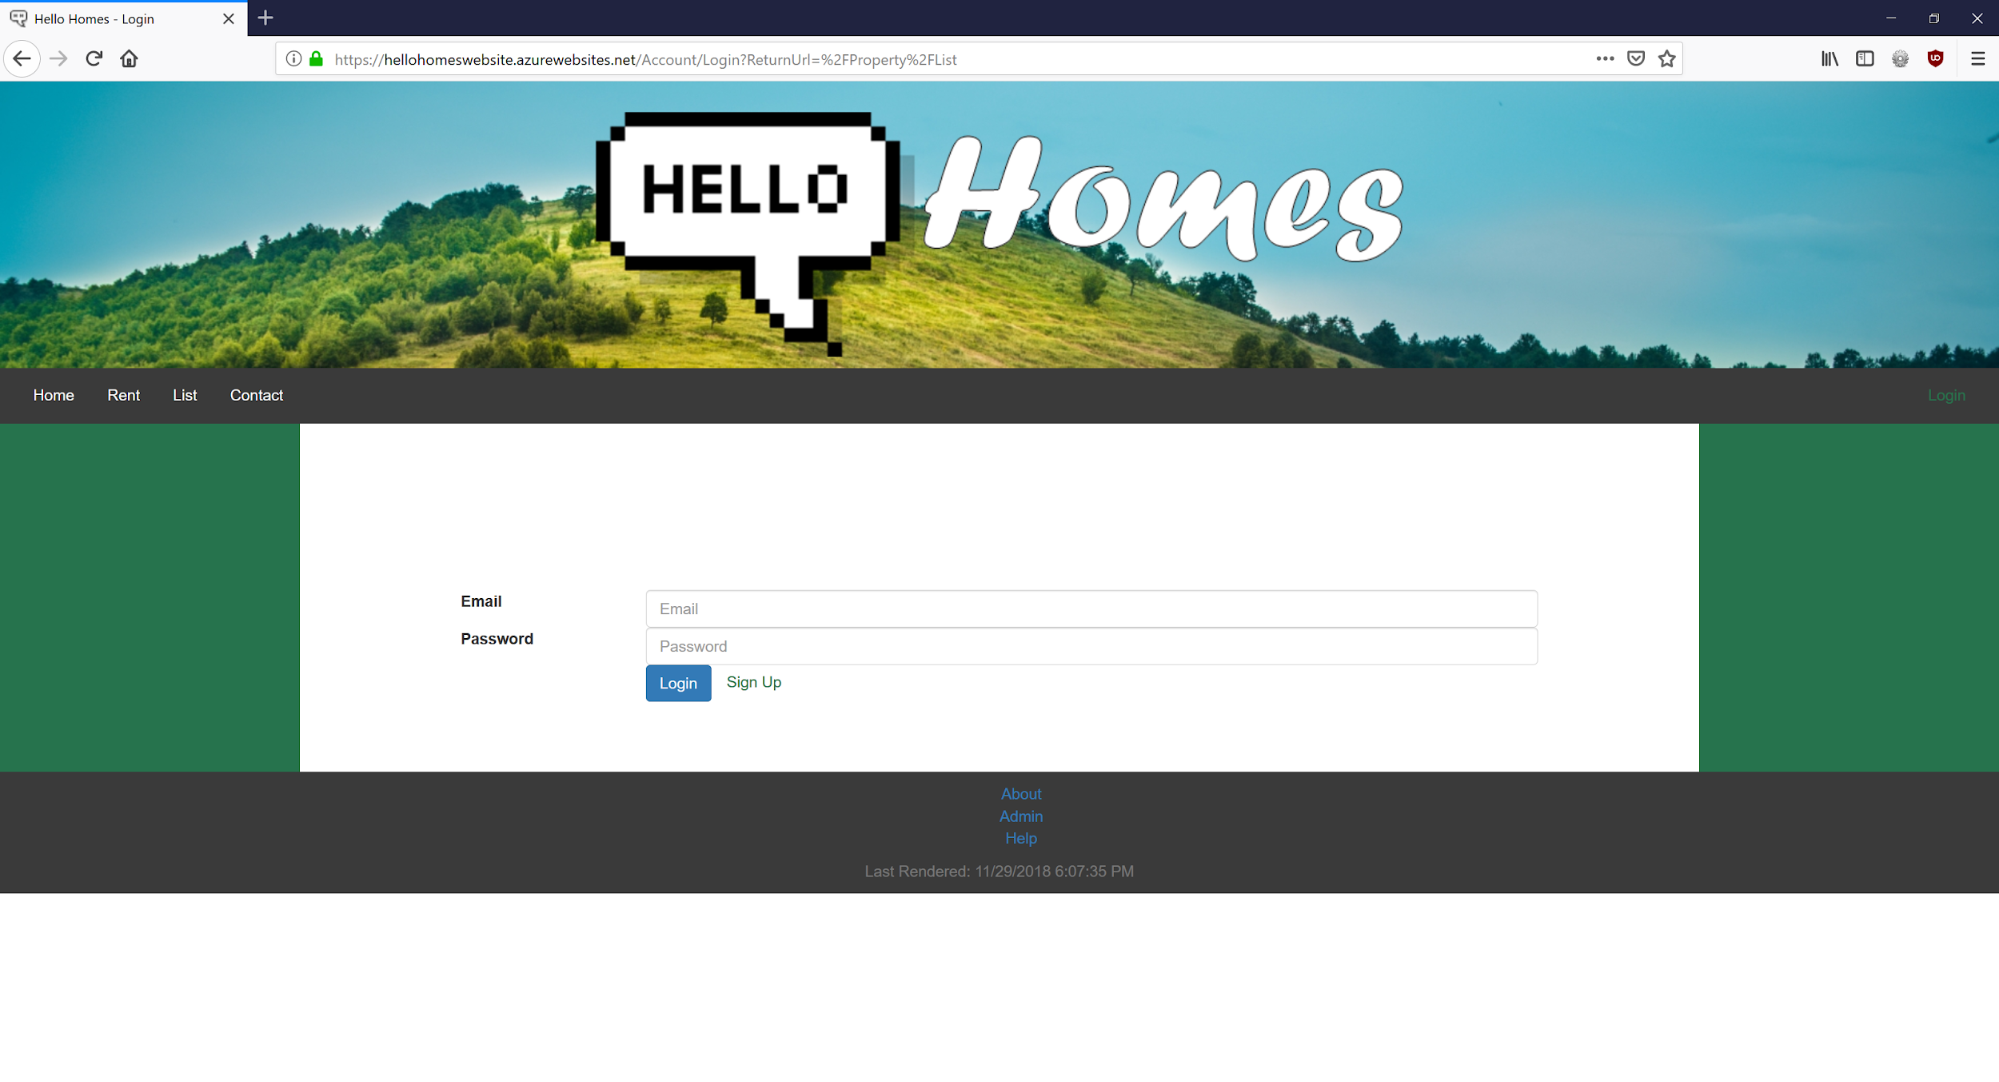
\includegraphics[width=0.8\textwidth]{figures/firefox.png}}
                \caption[Firefox Scaling]{There were some issues with the footer on Mozilla Firefox}
                \label{fig:firefox}
            \end{figure}

            \begin{figure}[!htb]
                \centering
                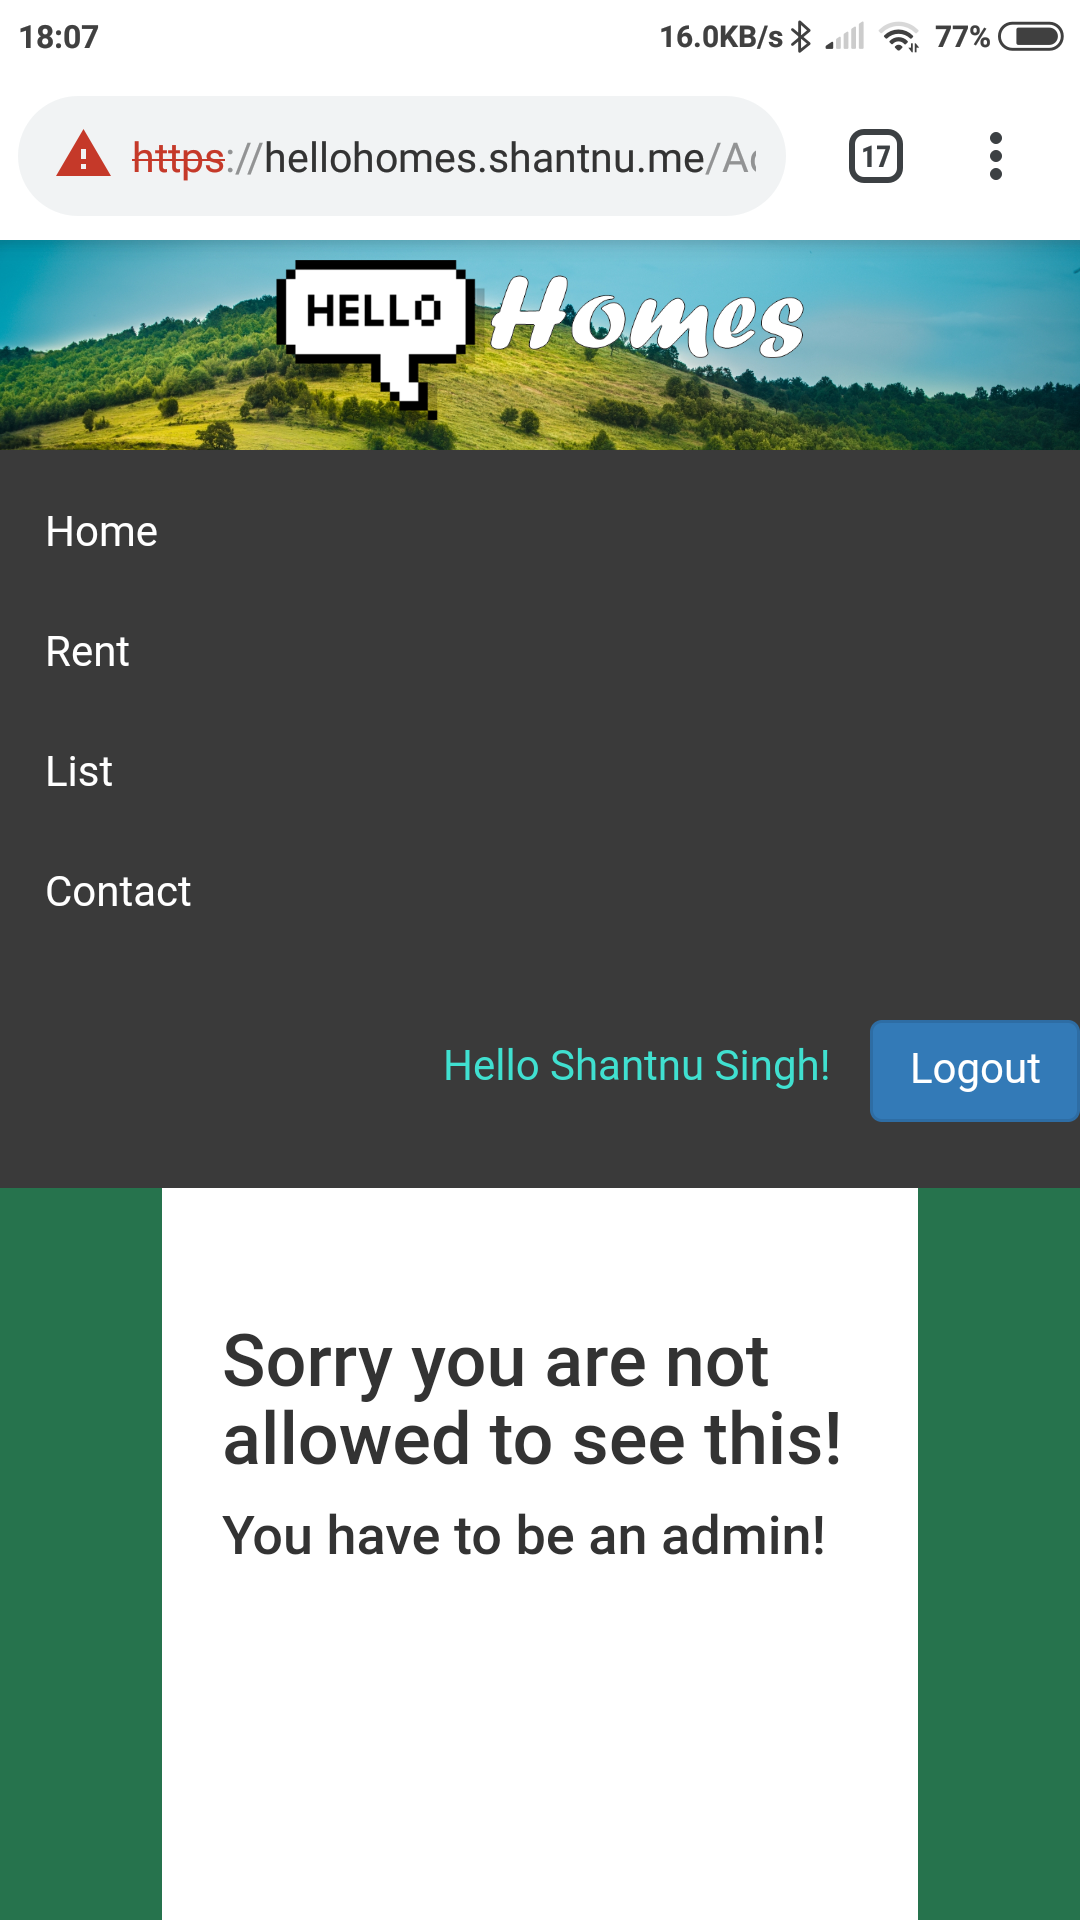
\includegraphics[width=0.4\textwidth]{figures/android.png}
                \caption[Android Scaling]{The navigation bar adjusted automatically on an Android phone}
                \label{fig:android}
            \end{figure}

            \begin{figure}[!htb]
                \centering
                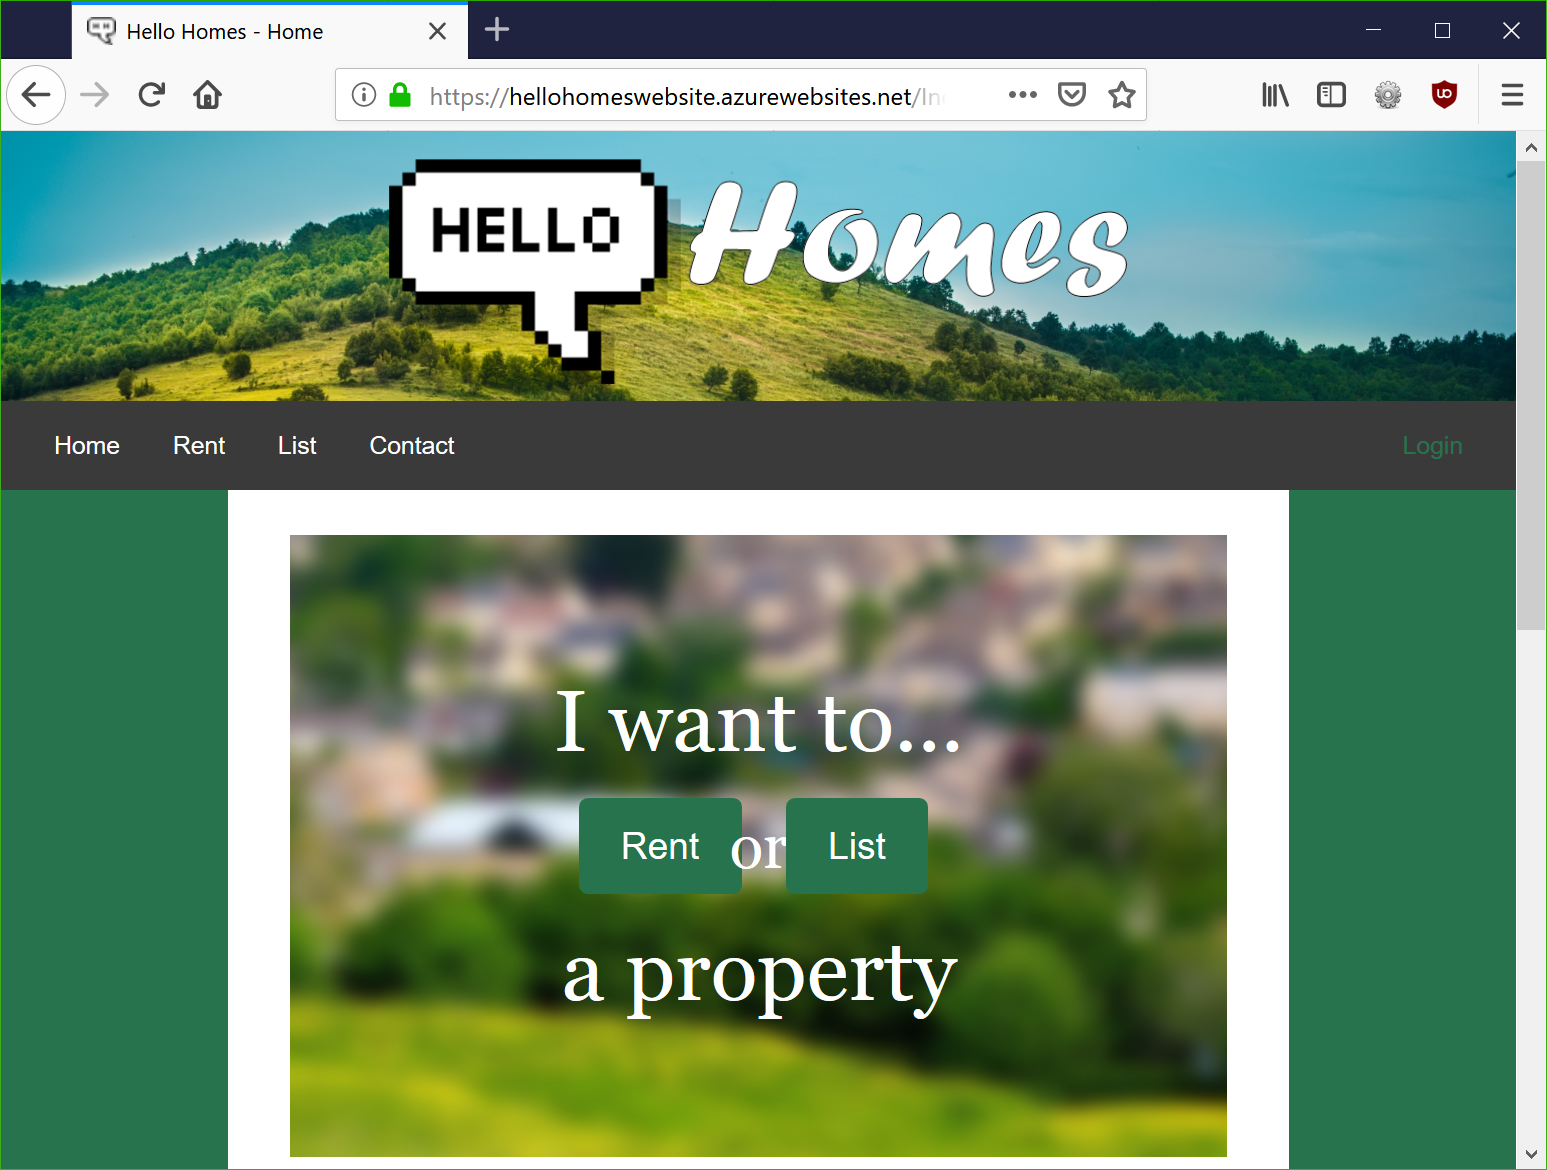
\includegraphics[width=0.8\textwidth]{figures/small_window.png}
                \caption[Small Window]{There were some issues with scaling on a small window}
                \label{fig:small_display}
            \end{figure}

    \subsection{Logic Testing}
        \paragraph{}
            User inputs on the site have to be tested to ensure they are correct. This includes making sure they are in the correct format, that they do not break application logic and are not missing when they shouldn't be. When there is an error on input, we have used Razor page’s ModelState functionality to display the relevant error to the user. We have shown one example of this.

        \paragraph{}
            Safeguards we have added to user input include:
            \begin{itemize}\itemsep 0pt
                \item Making sure required fields are not left empty
                \item Making sure a user does not sign up with an existing Email
                \item Making sure phone numbers and Emails are in the correct format - this was done using regular expressions and built in libraries on ASP.NET
            \end{itemize}

        \paragraph{}
            Other safeguards we have added are:
            \begin{itemize}\itemsep 0pt
                \item Displaying a default thumbnail if the property doesn't have an image
                \item 404 pages when a user accesses a page that doesn't exist
            \end{itemize}

            \begin{figure}[!htb]
                \centering
                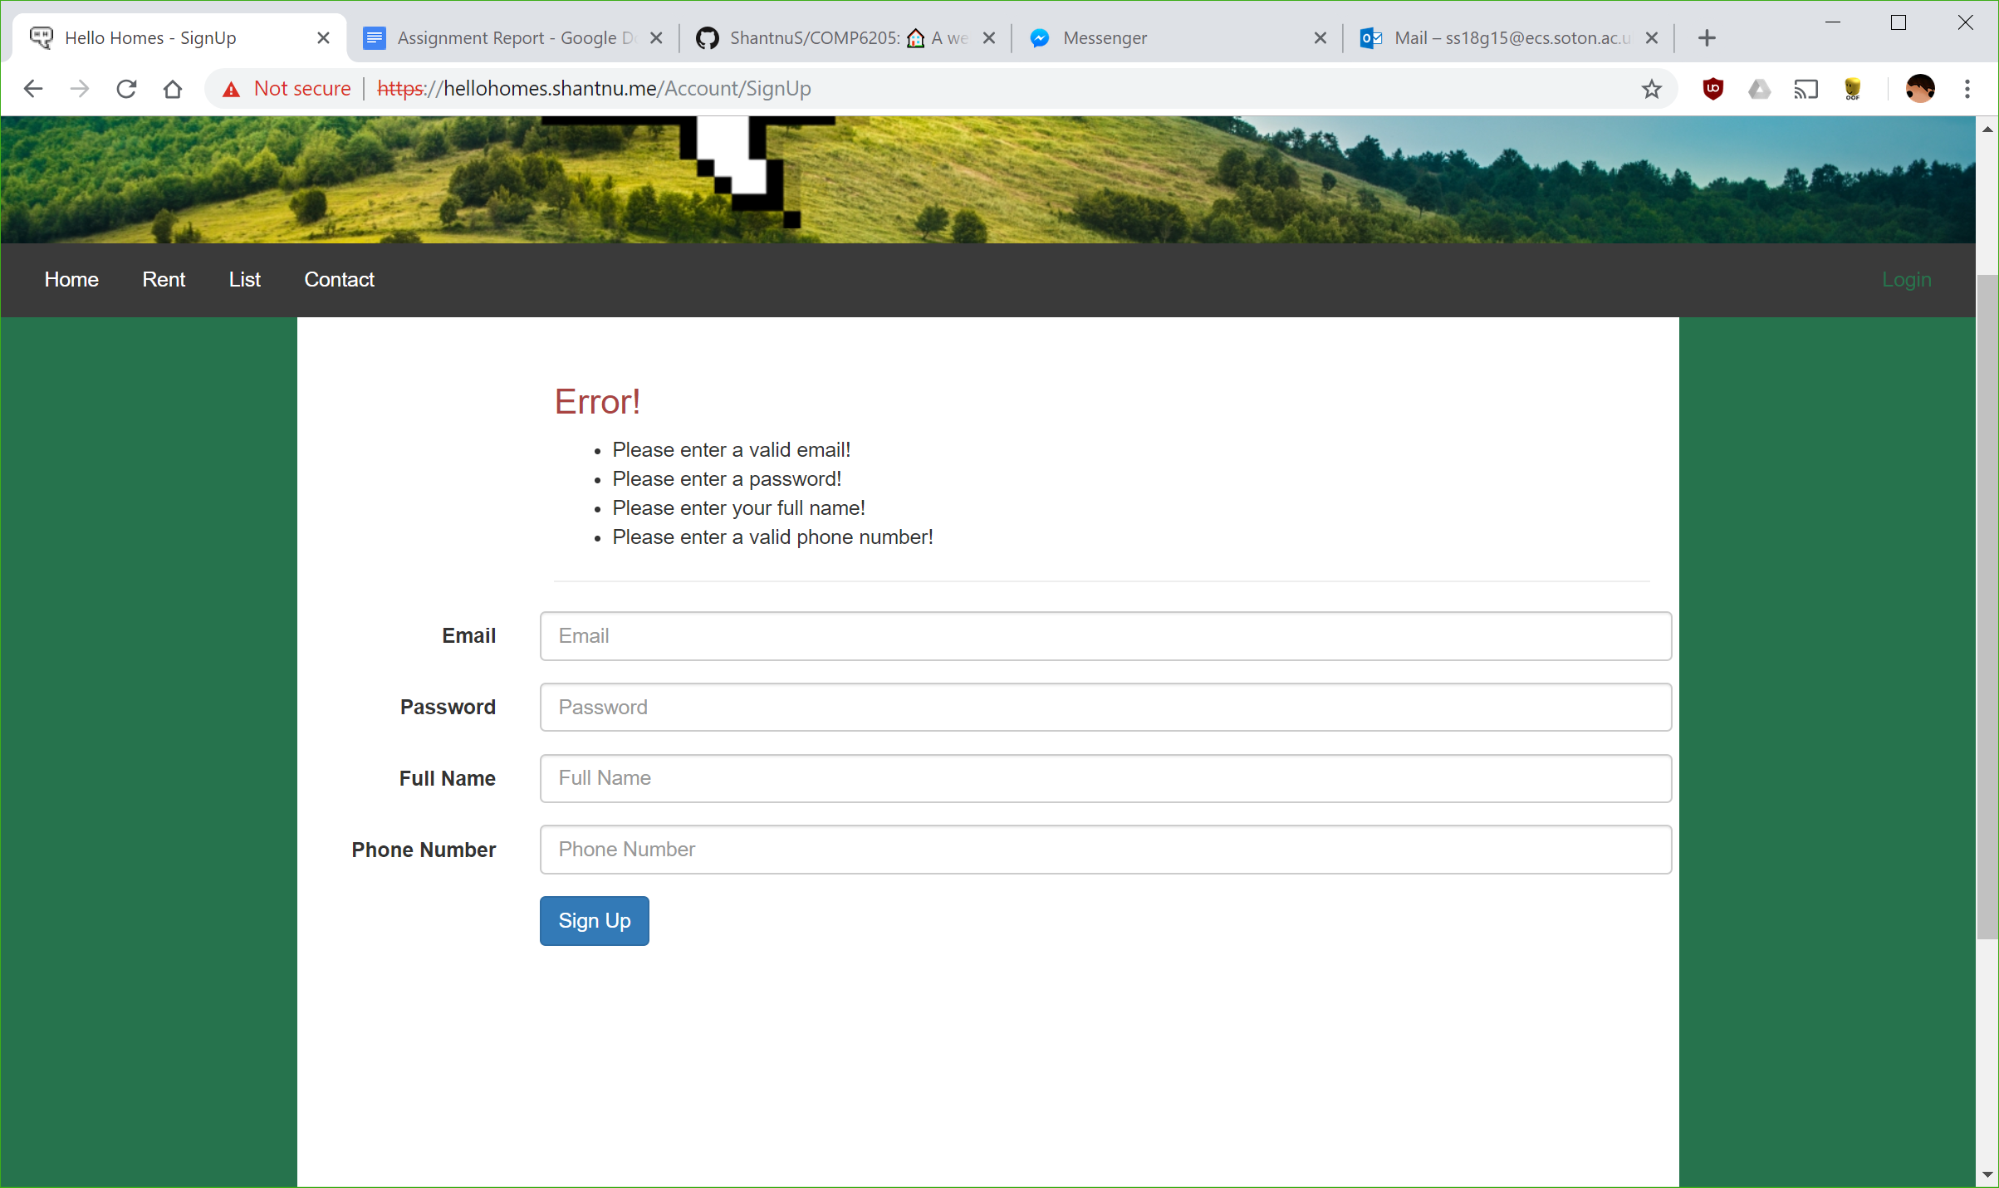
\includegraphics[width=0.8\textwidth]{figures/logic_error.png}
                \caption[Logic Error]{Example of how user input errors are displayed}
            \end{figure}

\FloatBarrier
\section{Extensions}
    \subsection{Deploying to Azure}
        \paragraph{}
            With Visual Studio 2017, it is very easy to deploy a Razor pages website to Microsoft Azure \cite{azure_tutorial}.
            This allows the app to be accessible from anywhere and since it is a Platform-as-a-Service (PaaS), there is no over/under-provisioning.
            Another reason to use Azure was that students get £150 of free credit upon joining, which is ideal to test our prototype website.

        \paragraph{}
            To deploy to Azure, we could simply right click on the project and click “publish”.
            After this we could set-up the deployment name and the SQL database we’d like to use - generating their tables using the migration and deploy the application.

        \paragraph{}
            Furthermore, we could also set-up a custom domain by adding a CNAME record on our domain’s DNS records.
            Since we already had a namecheap domain from a previous project, we could add a record for \href{https://hellohomes.shantnu.me/}{hellohomes.shantnu.me} and verify this CNAME on the Azure portal.
            After this the website was accessible from anywhere in the world.
            However, one issue was that the website uses ‘https’ but we haven’t configured an SSL certificate.
            This means a warning is displayed before connecting to the website.

            \begin{figure}[!htb]
                \centering
                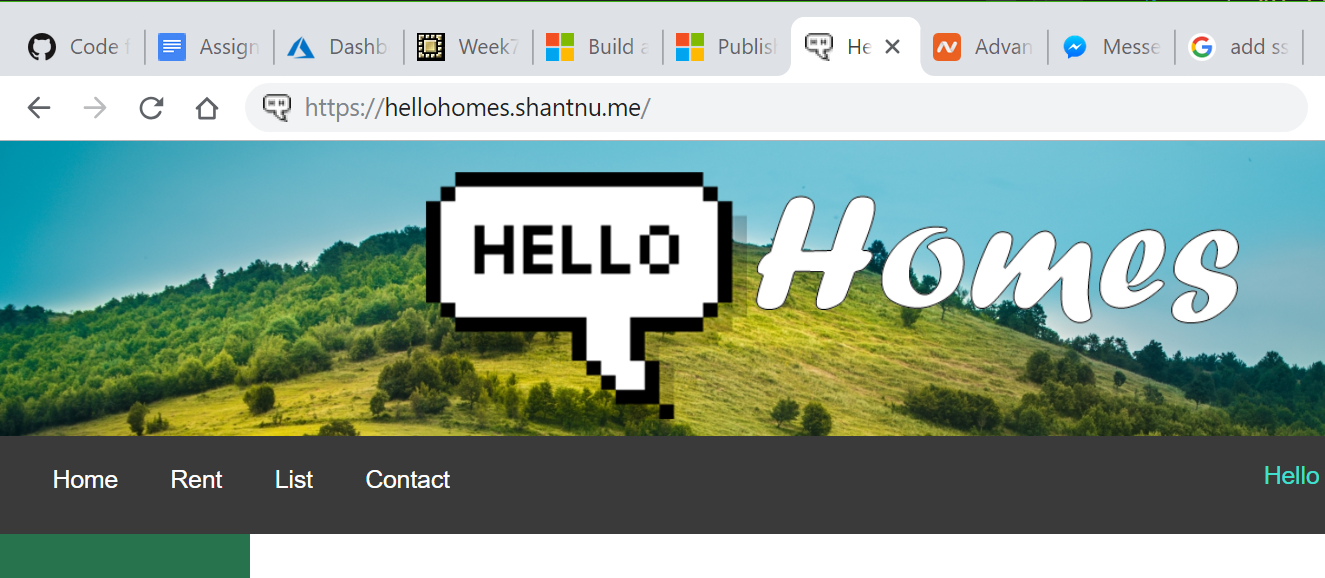
\includegraphics[width=0.8\textwidth]{figures/custom_domain.png}
                \caption[Custom Domain]{The web app hosted on a custom domain}
                \label{fig:custom_domain}
            \end{figure}

        \paragraph{}
            Apart from greater availability, another great advantage of Azure was the performance monitoring tools it provides.
            There is also an option to create alerts if there are any issues with the website, such as high CPU usage or downtime.

            \begin{figure}[!htb]
                \centering
                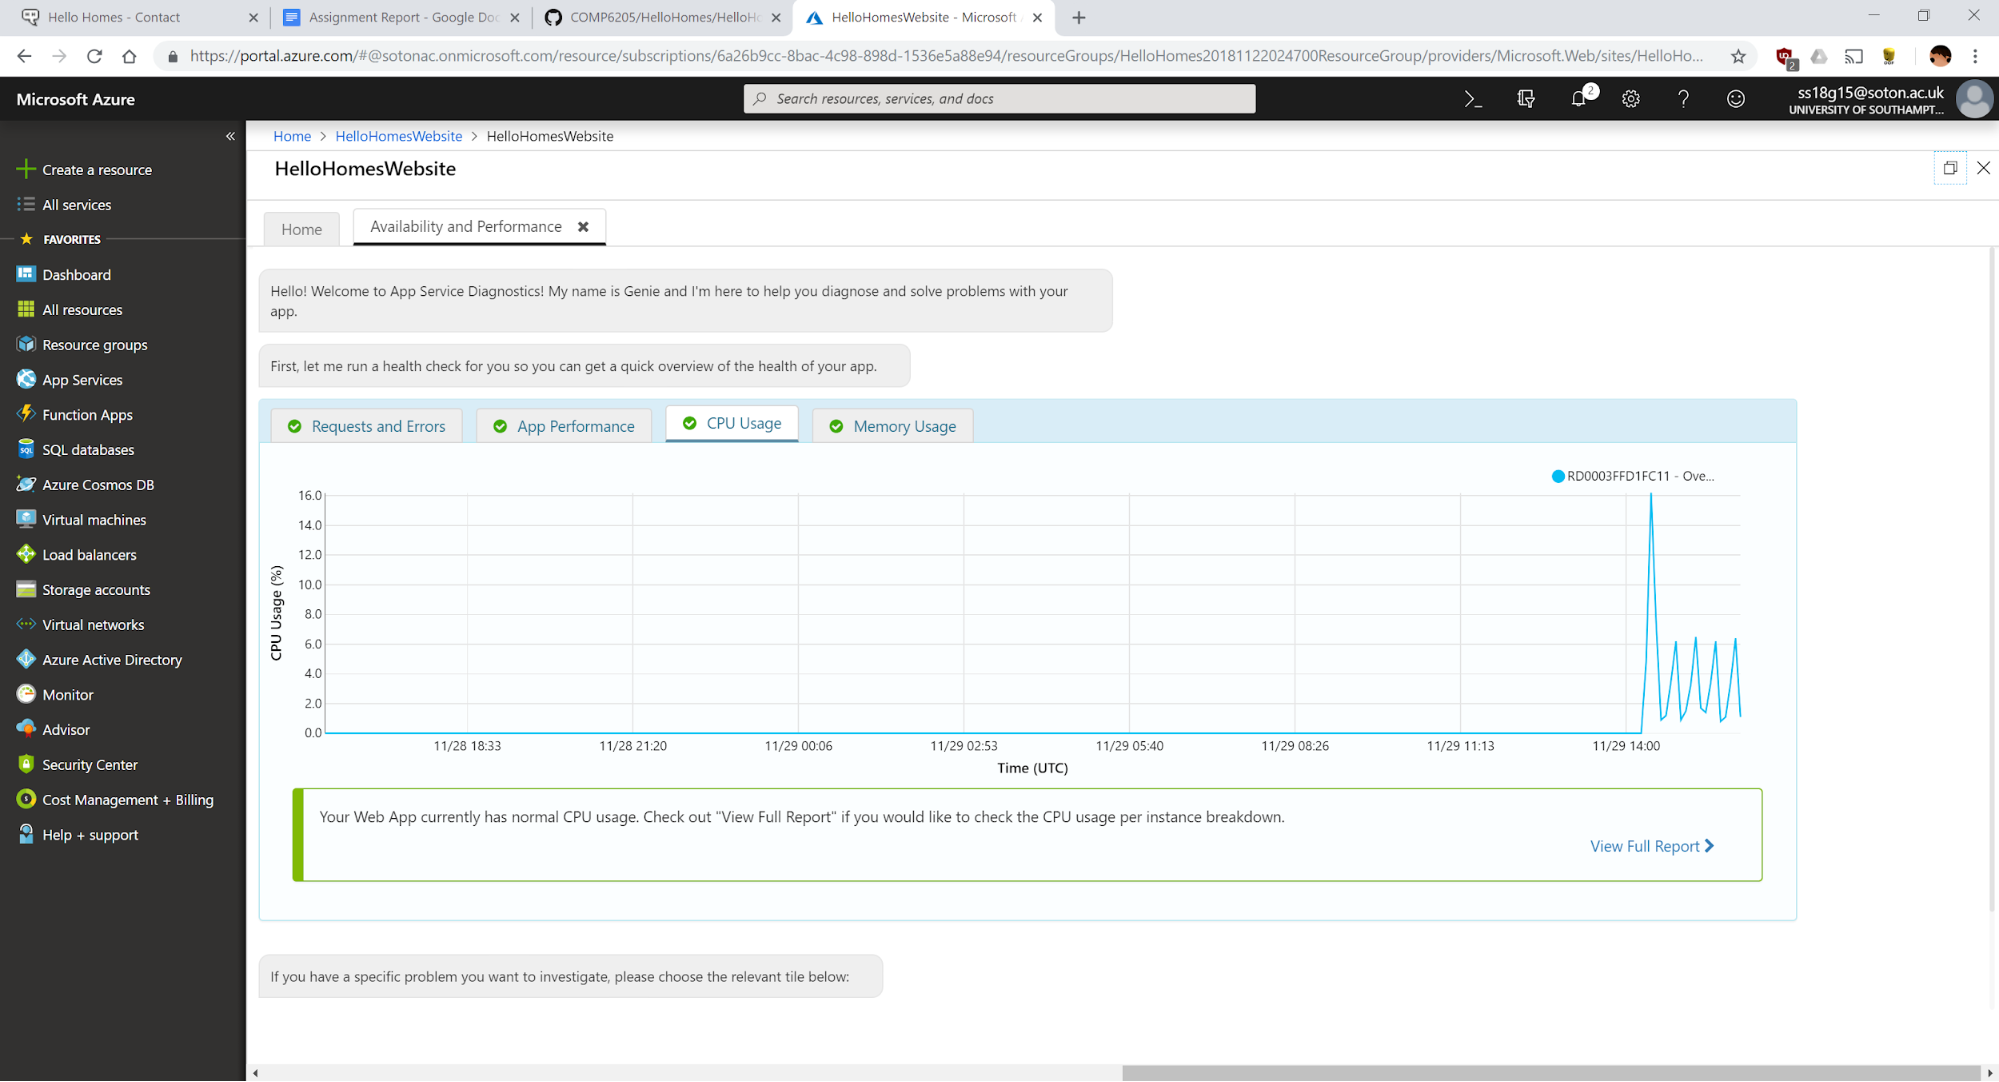
\includegraphics[width=0.8\textwidth]{figures/web_diagnostics.png}
                \caption[Performance Monitoring]{Azure provides a range of tools to monitor performance}
            \end{figure}

\FloatBarrier
\section{Critical Evaluation}
    \paragraph{}
        A problem arose at the start of the coursework due to the platform dependency of Visual Studio 2017 - however, once a Windows environment with the required software installed was readily available to both members, the tools proved simple to learn and highly effective.
        Visual Studio is a fully featured IDE that is well constructed to make the .NET framework easy to use, with basic features such as the automatic creation of the associated \texttt{.cshtml.cs} file for each page making development significantly easier.
        More advanced features such as IntelliSense were indispensable, providing invaluable information on both formal mistakes, such as missing \texttt{using} directives, and coding style related issues.

    \paragraph{}
        As a framework, ASP .NET has several benefits over it's competitors - \texttt{node.js} being the one we had experience in.
        It boasts tighter integration with the layout markup due to the use of \texttt{.cshtml} markup rather than \texttt{.html}, which is a significant quality of life improvement for elements like forms, where the passing of form field data to the controller is handled automatically.
        The custom markup format also allows page design more simple through the use of embedded code, allowing convenient notations such as the automatic display of variables: a feature which is used extensively in the \texttt{List.cshtml} and \texttt{Rent.cshtml} pages.
        It's integration with Visual Studio IDE is also a boon that other frameworks lack, at least to the extent that ASP .NET has, with tools such as the SQL database viewer allowing for extremely easy and effective debugging.

    \paragraph{}
        The major drawback of the framework was the learning curve: a new markup format and an unfamiliar language, paired with it's documentation being primarily written by Microsoft, made for an unforgiving experience towards the beginning of the coursework.
        However, this disadvantage was a moot point after the first few weeks, and the overall ease of use and fully featured development environment more than made up for the initial difficulty.

\newpage
\begin{thebibliography}{1}
    \bibitem{request_verification}
        "Request Verification in Razor Pages | Learn Razor Pages", Learnrazorpages.com, 2018. [Online]. Available: https://www.learnrazorpages.com/security/request-verification. [Accessed: 29- Nov- 2018]
    \bibitem{azure_tutorial}
        "Publish an ASP.NET Core app to Azure with Visual Studio", Docs.microsoft.com, 2018. [Online]. Available: https://docs.microsoft.com/en-us/aspnet/core/tutorials/publish-to-azure-webapp-using-vs?view=aspnetcore-2.1. [Accessed: 29- Nov- 2018]
    \bibitem{youtube_tutorial}
        "Building Basic Web App from Scratch with ASP.NET Core 1.0", YouTube, 2018. [Online]. Available: https://www.youtube.com/watch?v=4xhardjp6q0. [Accessed: 29- Nov- 2018]
    \bibitem{lynda_tutorial}
        J. Chadwick, "Creating Razor Pages", Lynda.com, 2018. [Online]. Available https://www.lynda.com/ASP-NET-tutorials/Creating-Razor-Pages/630622/679588-4.html. [Accessed: 29- Nov- 2018]
    \bibitem{ms_razor_docs}
        "Introduction to Razor Pages in ASP.NET Core", Docs.microsoft.com, 2018. [Online]. Available: https://docs.microsoft.com/en-gb/aspnet/core/razor-pages/. [Accessed: 29- Nov- 2018]
    \bibitem{dbcontext_tutorial}
        "Modifying data via the DbContext | Learn Entity Framework Core", Learnentityframeworkcore.com, 2018. [Online]. Available: https://www.learnentityframeworkcore.com/dbcontext/modifying-data. [Accessed: 29- Nov- 2018]
\end{thebibliography}

\end{document}
